\documentclass[a4paper]{article}

%% Language and font encodings
\usepackage[english]{babel}
\usepackage[utf8x]{inputenc}
\usepackage[T1]{fontenc}
\usepackage{caption}
\usepackage{courier}

%% Sets page size and margins
\usepackage[a4paper,top=3cm,bottom=2cm,left=3cm,right=3cm,marginparwidth=1.75cm]{geometry}

%% Useful packages
\usepackage{amsmath}
\usepackage{graphicx}
\usepackage{amsfonts}
\usepackage[colorinlistoftodos]{todonotes}
\usepackage[colorlinks=true, allcolors=blue]{hyperref}
\usepackage{float}
\usepackage{enumerate}
\usepackage{caption}
\usepackage{subcaption}
\DeclareMathOperator*{\argmax}{arg\,max}
\DeclareMathOperator*{\argmin}{arg\,min}



\DeclareMathOperator{\E}{\mathbb{E}}

\setlength\parindent{0pt}

\title{Image Segmentation and Clustering techniques}
\author{Ding-Chih Lin}

\begin{document}
\maketitle

\begin{abstract}
This is the midterm report for the course of statistical computing. The topics presented here is \textbf{image segmentation} and \textbf{its related clustering techniques}. In the first section, I introduce the idea of image segmentation via some practical applications, and the classes of related techniques. In the second section, I formally elaborate the formulations of these related techniques: K-means Clustering, Hidden Markov Model and Spectral Clustering. In the next section, I design a simulation study to  see the performance for different cluster methods in different scenarios. In the last section, I utilize these methods to real world image data.

\end{abstract}


\section{Introduction}

In digital image processing and computer vision, image segmentation is the process of partitioning a digital image into multiple segments. The main goal of image segmentation is to simplify and alter the representation of an specific image into something which is meaningful or easier to analyze with. More precisely, image segmentation is the process of assigning a label to every pixel in an image such that pixels with the same label share certain characteristics.


\

Here I present some practical applications of image segmentation
\begin{itemize}
	\item Tumor segmentation from medical images such as  X-ray, MR image and CT image.
	\item Object detection for autonomous vehicles or satellite.
	\item Color quantization, the process of reducing the number of colors in an image without loss of quality, in the research of data compression.
	\item Optical character recognition (OCR) for text-based image.
\end{itemize}


Several algorithms and techniques for image segmentation have been developed using domain-specific knowledge to solve segmentation problems in that specific application area. Segmentation techniques can be categorized into three classes: \textit{graph-based}, \textit{cluster-based} and \textit{deep learning-based} methods. In this midterm project, I will utilize K-means clustering algorithm,  spectral cluster algorithm and Hidden Markov Model.

\section{Related Techniques}

\subsection{K-means Clustering}

Given the data $x = \{ x_1, ..., x_n\}$ and an initial set of $k$ means $m_1^{(1)}, ..., m_k^{(1)}$, the algorithm proceeds by alternating between the following two steps
\begin{enumerate}
	\item Assign each observation to the cluster with the nearest mean in $t$ step
		\begin{equation}
			S_t^{(t)} = \{ x_p : || x_p - m_i^{(t)} ||^2 \leq || x_p - m_j^{(t)} ||^2  , \quad \forall 1\leq j \leq k \}, \quad p = 1, ..., n
		\end{equation}
	\item Recalculate means for observation assigned to the new cluster in $t$ step
		\begin{equation}
			m_i^{(t+1)} = \frac{1}{ | S_t^{(t)} | } \sum (x_j)
		\end{equation}
\end{enumerate}
The above algorithm proceeds until the assignments no longer change.

\

The most commonly used methods to decide an initial set of $k$ means are \textit{Random Partition} and \textit{Forgy method}. The random partition method randomly assigned a cluster to each observation and calculate the initial set of $k$ means, then proceeds the algorithm. The Forgy method randomly choose $k$ observations from the data $x$ and use their value as the initial set of $k$ means, then proceeds the algorithm.

\subsection{Spectral Clustering}

Spectral clustering is a technique with roots in graph theory. This approach is used to identify the clusters of nodes in a graph based on the edges connecting them. It utilize information from the eigenvalues, which is so-called spectrum, of the similarity matrix built from the graph. Different from K-means using the absolute locations, it utilize affinity to determine what points fall under which cluster.

\

Given the data $x = \{ x_1, ..., x_n\}$, it can be transformed to a complete undirected graph $G(V, E)$ with corresponding similarity $w_{ij}$, $i,j=1, ..., n$. The similarity matrix may be defined as a symmetric matrix $W = [w_{ij}]_{i,j=1,...,n}$. The element of $W$ is greater than zero and represents a measure of the similarity between data point $x_i$ and $x_j$. The general approach to spectral clustering is to use a standard clustering method (for example, K-means) on relevant eigenvectors of a Laplacian matrix of $G$. There are several ways to define Laplacian matrix with different interpretations, and then these clustering results are applicable in different scenarios.

\

Define the Laplacian matrix as 
\begin{equation}
	L = D-W
\end{equation}
where $D$ is the degree matrix and $W$ is the weight matrix of the graph. We usually use Gaussian kernel to define the graph edge weight connecting two nodes $i$ and $j$
\begin{equation}
		w_{ij} = e^{\frac{- || x_i - x_j || ^2_{2}}{\sigma^2}}
\end{equation}


Then, define the symmetric normalized Laplacian matrix as 
\begin{equation}
	L^{\mbox{norm}} = D^{-\frac{1}{2}} L D^{-\frac{1}{2}}  =I - D^{-\frac{1}{2}} W D^{-\frac{1}{2}}
\end{equation}

A popular spectral clustering technique is \textbf{normalized cuts algorithm}, proposed in \textit{normalized cuts and image segmentation, Jianbo Shi and Jitendra Malik}. It partition data points into two sets based on the eigenvector corresponding to the second-smallest eigenvalue of the $L^{\mbox{norm}}$.

\

The algorithm of spectral clustering is described as follow

\begin{enumerate}
	\item Calculate the Laplacian matrix $L$
	\item Calculate the first $k$ eigenvectors
	\item Consider the matrix formed by the first $k$ eigenvectors; the $l$-th row defines the features of graph node $l$
	\item Using K-means technique to cluster the graph nodes based on these feature defined in (3)
\end{enumerate}

Basically, spectral clustering techniques utilize eigenvalue of the weight matrix to perform dimension reduction before clustering in lower dimensions. It is known as segmentation-based object categorization.


\subsection{Hidden Markov Model}

Hidden Markov Model is a discrete-time doubly embedded stochastic process, where the process $X$ being modeled is assumed to be a Markov process with unobserved (hidden) states $Y$ that depends on $X$.  The goal is to learn about $X$ in order to observe or obtain $Y$.

\

Assume we observe sequential data $x = \{ x_1, ..., x_t \}$ which is assumed to be a Markov process. $u$ is generated by a chain of hidden states $s = \{ s_1, ..., s_T\}$, and each $s_t$ can take $M$ states with initial probability $\pi_k$, $k=1, ..., M$. The distribution of $x$ conditional on $s$ is represented as $b_k(x)$, which is called emission probability
\begin{equation}
	x_t | s_t = k \sim b_k (x_t)
\end{equation}


The changes of states between consecutive hidden state is specified by transition probability 
\begin{equation}
	a_{k,l} = P(s_{t+1} = l | s_t = k) 
\end{equation}
and denote the transition probability matrix by $A$. We can further assume time-homogeneous transition probabilities property to make the structure of $A$ simpler.  

\

The goals now can be summarized into two parts based on HMM
\begin{itemize}
	\item Parameter estimation: $\hat{\lambda} = \{ \hat{\pi}_k, \hat{b}_k(x), \hat{a}_{k,l} \}  = \argmax_{\lambda} P(x | \lambda)$ via EM algorithm 
	\item Cluster problem: probabilities of the underlying states, given the observations, $P(s|x)$.
	\begin{equation}
		\hat{s} = \argmax_s P(s | \lambda, x)
	\end{equation}
\end{itemize}

In order to solve the first problem, we can make parametric assumptions of the emission probabilities $b_k(x_t)$, which normally distributed with parameters $\mu_k$ and $\sigma_k^2$. Therefore, the parameters in HMM are 
\begin{equation}
	\lambda = \{ \pi_k, \mu_k, \sigma_k^2, a_{k,l} : k = 1, ..., M \}
\end{equation}

$\lambda$ can be estimated from the observed likelihood function, but it is unreasonable since it involves $M^T$ possible paths. However, we can utilize backward and forward algorithms to simplify the calculation of observed likelihood given $\lambda$.

\

Ignoring some derivation of forward and backward recursive calculation, the observed data likelihood can be represented as forward probability $\alpha_k (t)$ and backward probability $\beta_k (l)$
\begin{align}
\begin{split}
	P(x_1, ..., x_T)  &  = \sum_{k=1}^{M} \alpha_k (T) = \sum_{k=1}^{M} \beta_k (1) P(x_1 | s_1 = k) P(s_1 = k) \\
	& = \sum_{k=1}^{M} \alpha_k(t) \beta_k (t)
\end{split}
\end{align}

\

We have prepared everything we need in the estimation of $\lambda$ through EM algorithm. The EM algorithm for HMM with Gaussian assumption is described as follows

\begin{itemize}
	\item \textbf{E-step}: evaluate $L_k(t)$ and $H_{k,l} (t)$ given $\lambda_{t-1}$, where
	\begin{equation}
		L_k(t) = P(s_t = k | x) = \frac{P(x, s_t = k )}{P(x)} =\frac{\alpha_k(t) \beta_k(t)}{\sum_{k=1}^{M} \alpha_k (t) \beta_k (t)} \\
	\end{equation}
	
	\begin{equation}
		H_{k,l} (t) = P(s_t=k, s_{t+1} = l | x) =\frac{\alpha_k (t) a_{k, l} b_l(y_{t+1}) \beta_l (t+1)}{\sum_{k=1}^{M} \alpha_k (t) \beta_k (t)}
	\end{equation}
	
	\item \textbf{M-step}: update parameters
		\begin{enumerate}
			\item For initial probability $\pi_k$ with constraint $\sum_{k=1}^{M} \pi_k = 1$
			\begin{equation}
				\hat{\pi}_k = \frac{L_k (1)}{\sum_{k=1}^{M} L_k(1)}
			\end{equation}
			
			\
			
			\item For transition probability $A = [a_{kl}]$ with constraint $\sum_{l=1}^{M} a_{kl} = 1$ for $k = 1, ..., M$
			\begin{equation}
				\hat{a}_{k,l} = \frac{\sum_{t=2}^{T} P(s_{t-1} = k, s_t = l | x, \lambda^{t-1})}{\sum_{l=1}^{M} \sum_{t=2}^{T} P(s_{t-1} = k , s_t = l | x, \lambda^{t-1})}  = \frac{\sum_{t=2}^{T} H_{k,l}(t)}{\sum_{t=1}^{M} \sum_{t=2}^{T} H_{k,l} (t)}
			\end{equation}
			
			
			\item For emission probability $b_{k}(x) = N(x_t | \mu_k, \sigma_k^2)$
			\begin{equation}
				\hat{\mu}_k = \frac{\sum_{t=1}^{T} L_k(t) x_t}{\sum_{t=1}^{T} L_k(t)}, \quad \hat{\sigma}^2 = \frac{\sum_{t=1}^{T} L_k(t) (x_t - \hat{\mu}_k)^2}{\sum_{t=1}^{T} L_k(t)}
			\end{equation}
		\end{enumerate}
\end{itemize}

Once the parameter estimated from EM algorithm reach the convergence condition, we can utilize HMM to cluster the dataset into $M$ groups. The detail for clustering with HMM and its variations is presented in \textit{Clustering Hidden Markov Models with Variational HEM, Coviello et al., Journal of Machine Learning Research, in 2014}. 

\section{Experimental Design}
In this section, I artificially design three scenarios, and make a $n= 1000$ simulation study to visualize the clustering results obtained from the methods in section 2. Beside the visualizations, I also provide the accuracy rate (random index) among $M = 200$ repeated random samples. The functions required to reproduce the same results are presented in \texttt{Simulation.py} and \texttt{tools.py} file on Github.

\subsection{Scenario one: two-dimensional independent normal distribution}

In the first scenario, consider the following data generating process with three clusters:

\begin{align}
	& x_{1k}, ..., x_{nk} \sim_{iid} N_2 (\mu_k,  \Sigma_k), \quad k = 1, 2, 3
\end{align}

\

where $\mu_1 = (1, 2)'$, $\mu_2 = (18, 5)'$, $\mu_3 = (5, 15)'$, 
$\Sigma_1 = \left( \begin{smallmatrix} 2&0\\ 0&2 \end{smallmatrix} \right)$, $\Sigma_2 = \left( \begin{smallmatrix} 2&0\\ 0&1 \end{smallmatrix} \right)$ and $\Sigma_3 = \left( \begin{smallmatrix} 5&0\\ 0&4 \end{smallmatrix} \right)$

\

The simulations from the DGP in equation (16) is presented in Figure 1. 

\begin{figure}[h!]
  \centering
  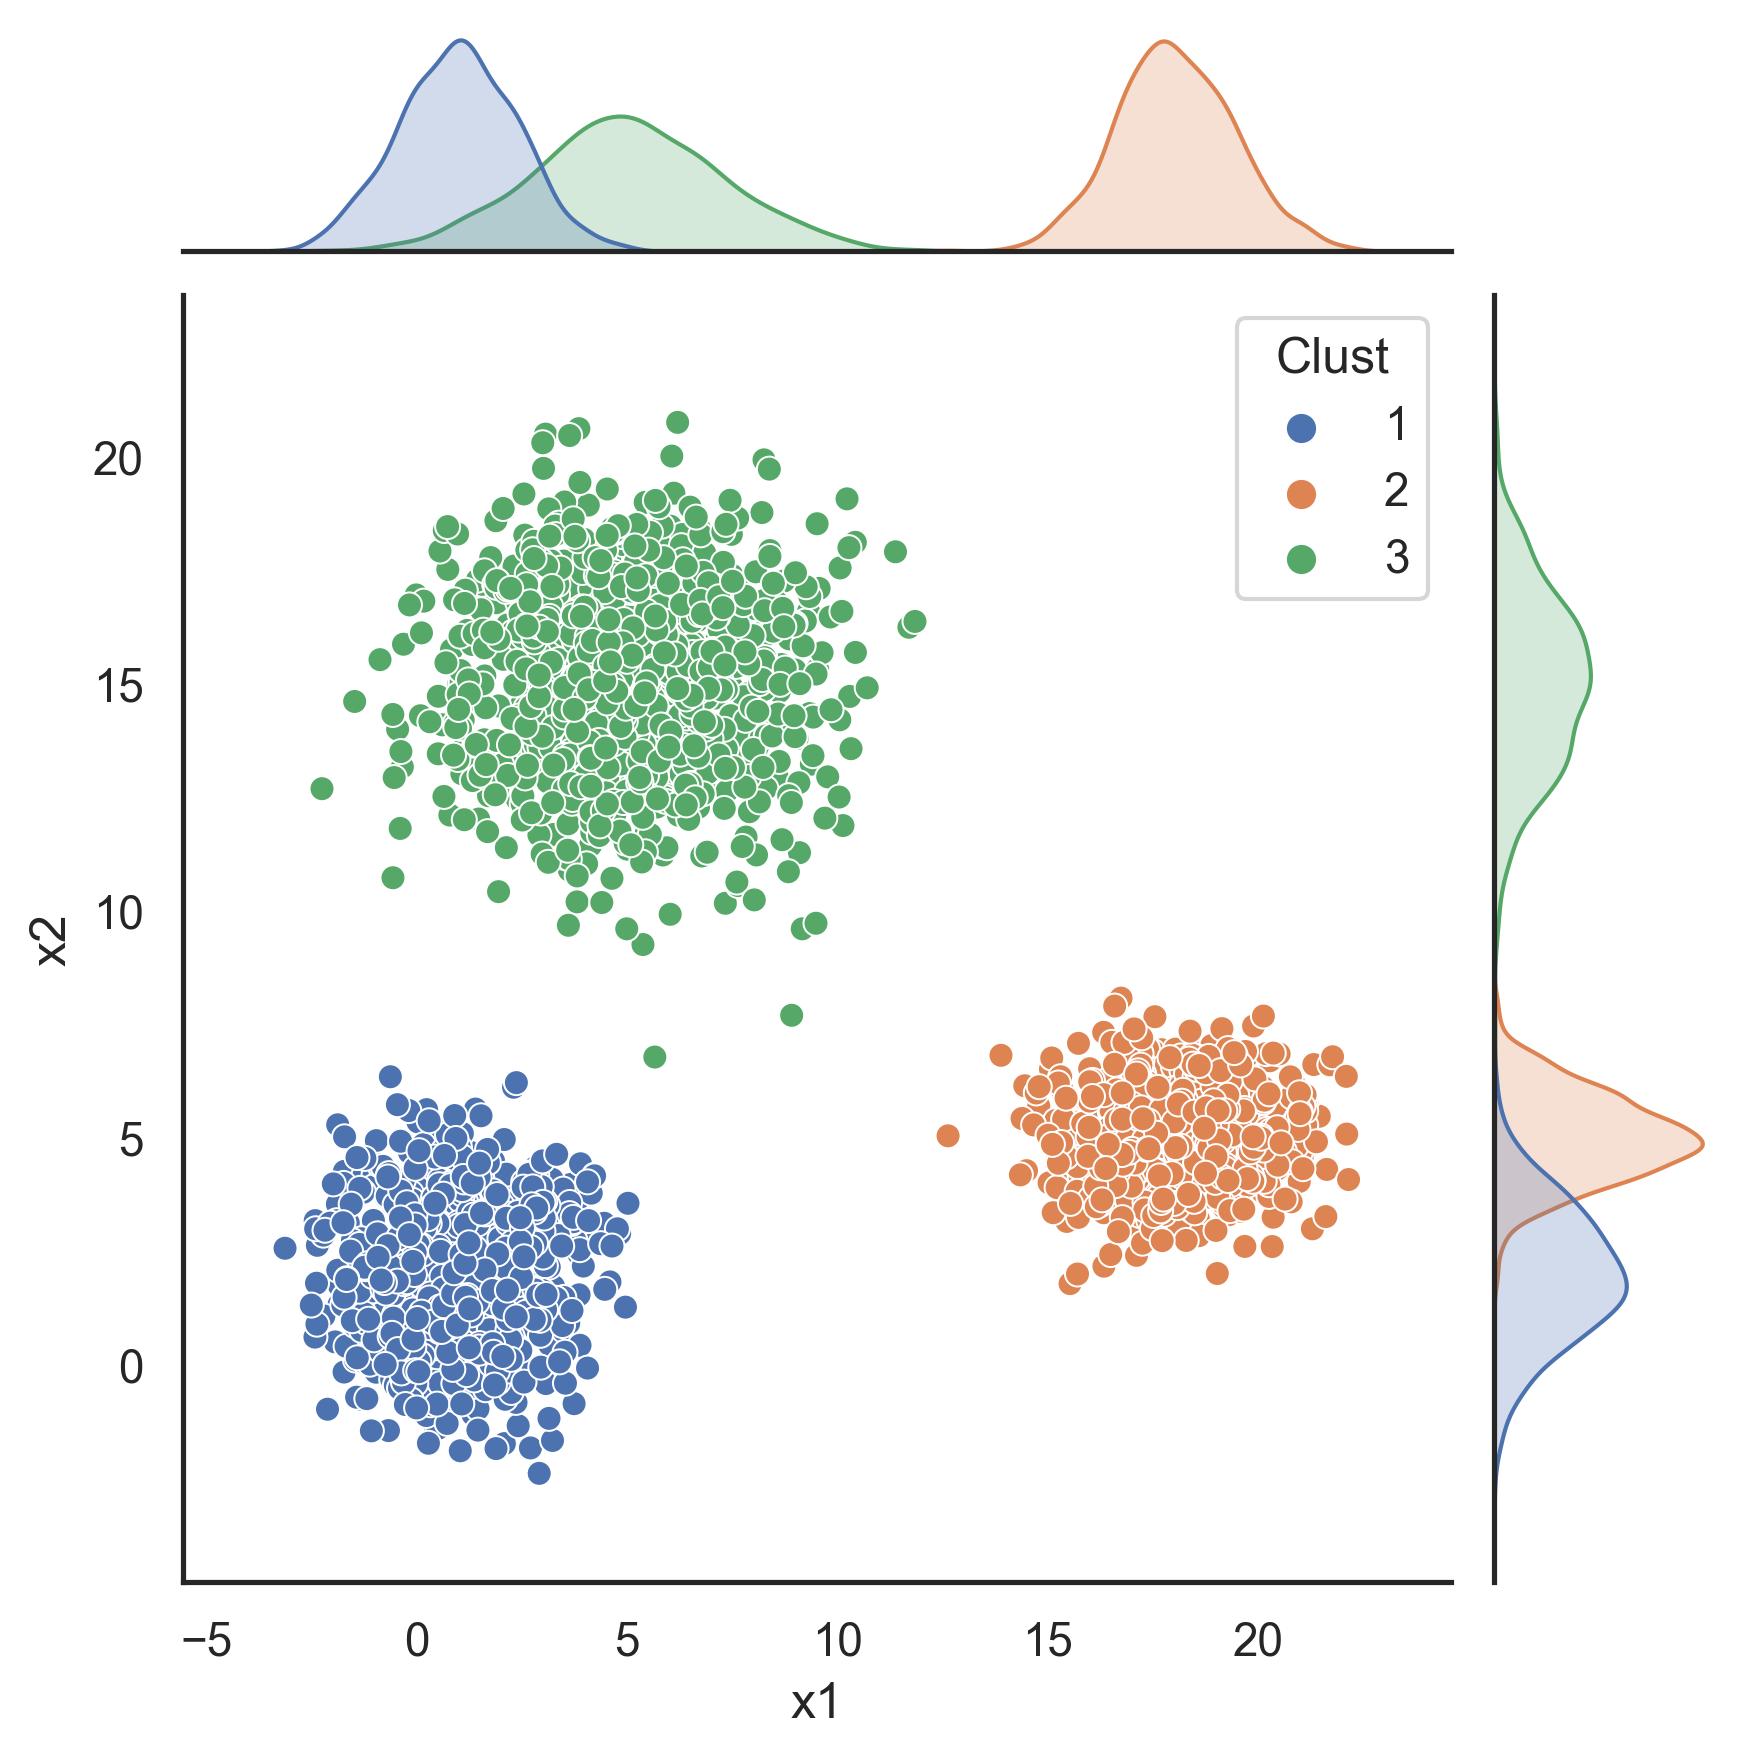
\includegraphics[width=0.45\linewidth]{../Simu_results/sen1.png}
  \caption{Simulation result from equation (16) and its true labels}
  \label{fig:sec}
\end{figure}

\

Next apply the K-means clustering, spectral clustering and HMM clustering method to the data we just generated, respectively. The cluster results are presented in Figure 2. By the fact that the three clusters are space-separated enough and the data in each cluster are independent. The performances of clustering are equally good as in these three methods.

\begin{figure}[h!]
  \centering
  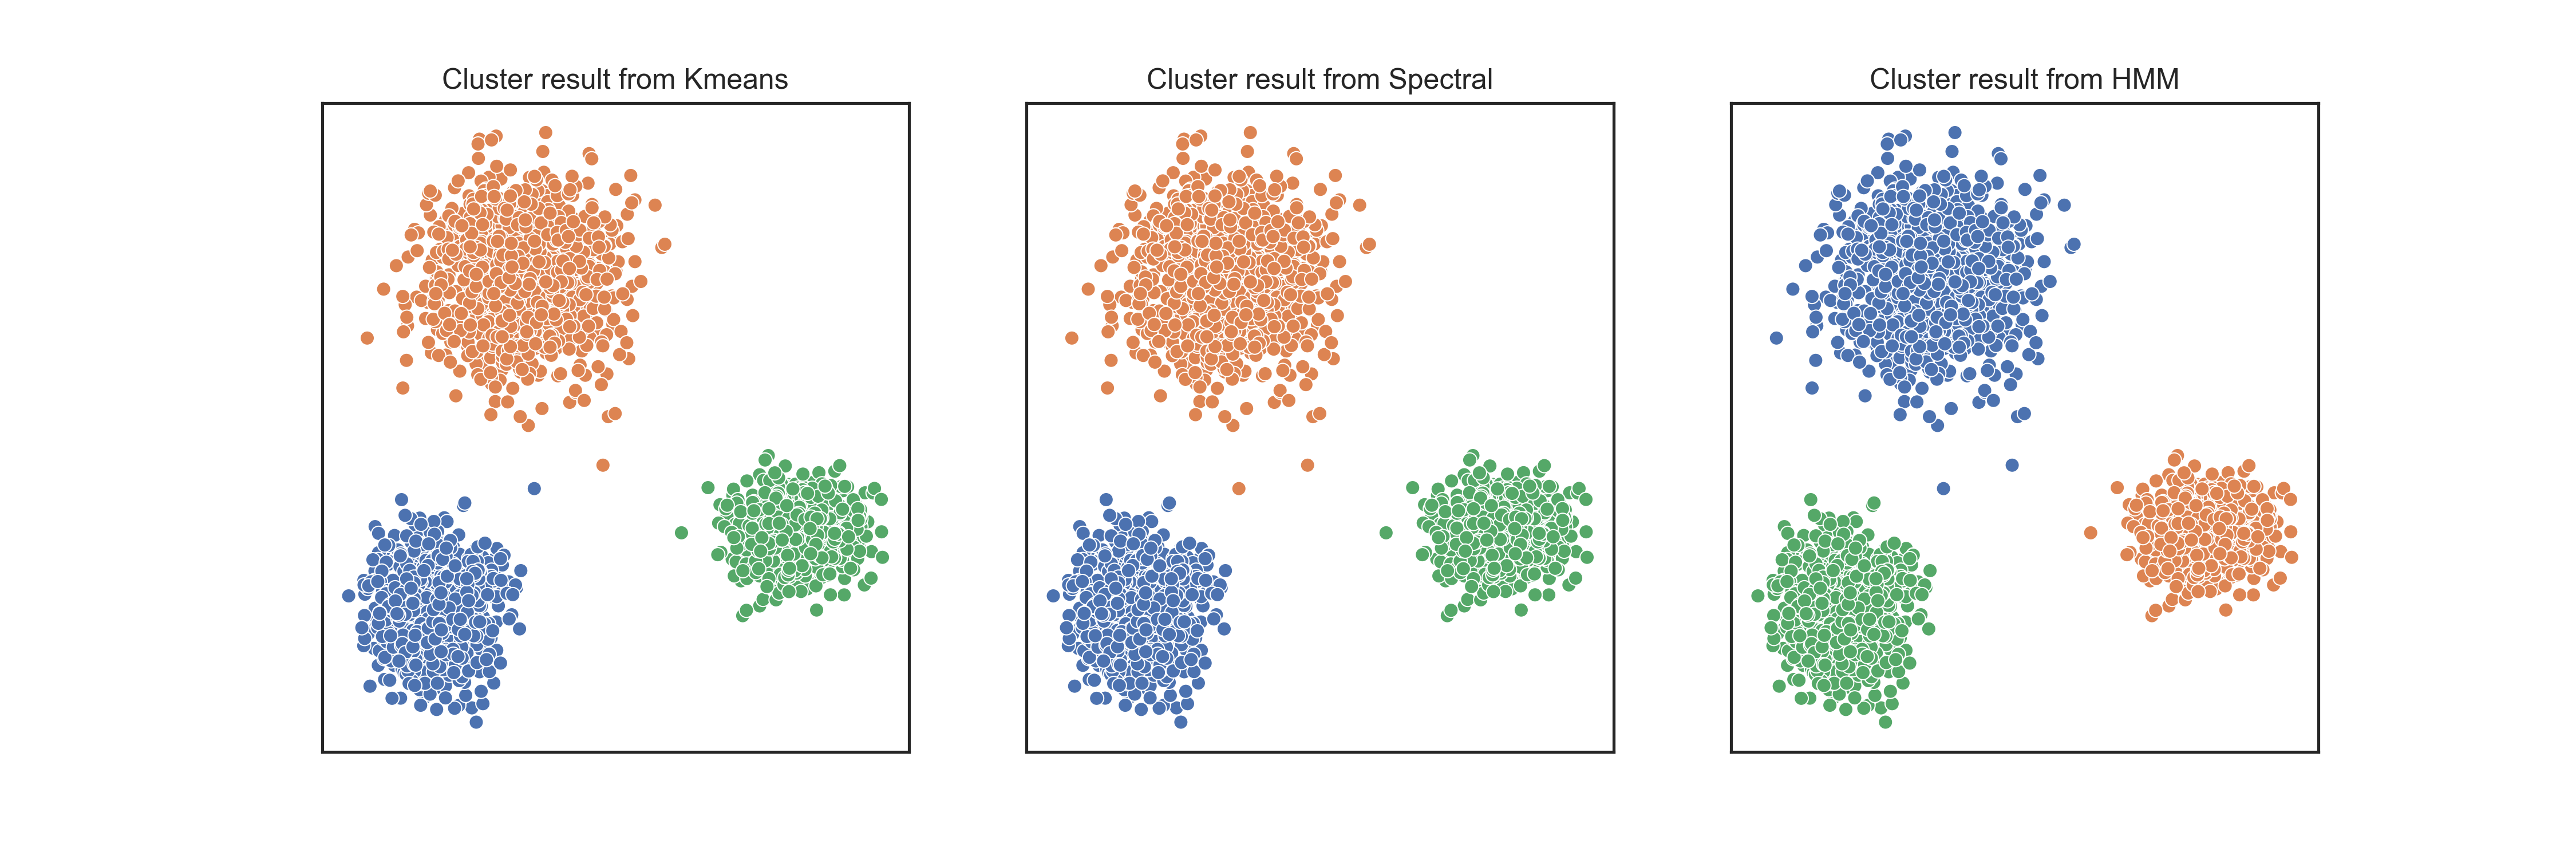
\includegraphics[width=0.8\linewidth]{../Simu_results/sen1_clust.png}
  \caption{Cluster results from K-means Clustering, Spectral Clustering and HMM in scenario 1}
  \label{fig:sec}
\end{figure}


\subsection{Scenario two: two-dimensional correlated normal distribution}

In the second scenario, consider the following data generating process with three clusters:

\begin{align}
	& x_{1k}, ..., x_{nk} \sim_{iid} N_2 (\mu_k,  \Sigma_k), \quad k = 1, 2, 3
\end{align}

\

where $\mu_1 = (1, 2)'$, $\mu_2 = (20, 20)'$, $\mu_3 = (10, 20)'$, 
$\Sigma_1 = \left( \begin{smallmatrix} 1&2\\ 2&1 \end{smallmatrix} \right)$, $\Sigma_2 = \left( \begin{smallmatrix} 6&6\\ 6&8 \end{smallmatrix} \right)$ and $\Sigma_3 = \left( \begin{smallmatrix} 6&6\\ 6&8 \end{smallmatrix} \right)$


\

The simulation from the DGP in equation (17) is presented in Figure 3. 

\begin{figure}[h!]
  \centering
  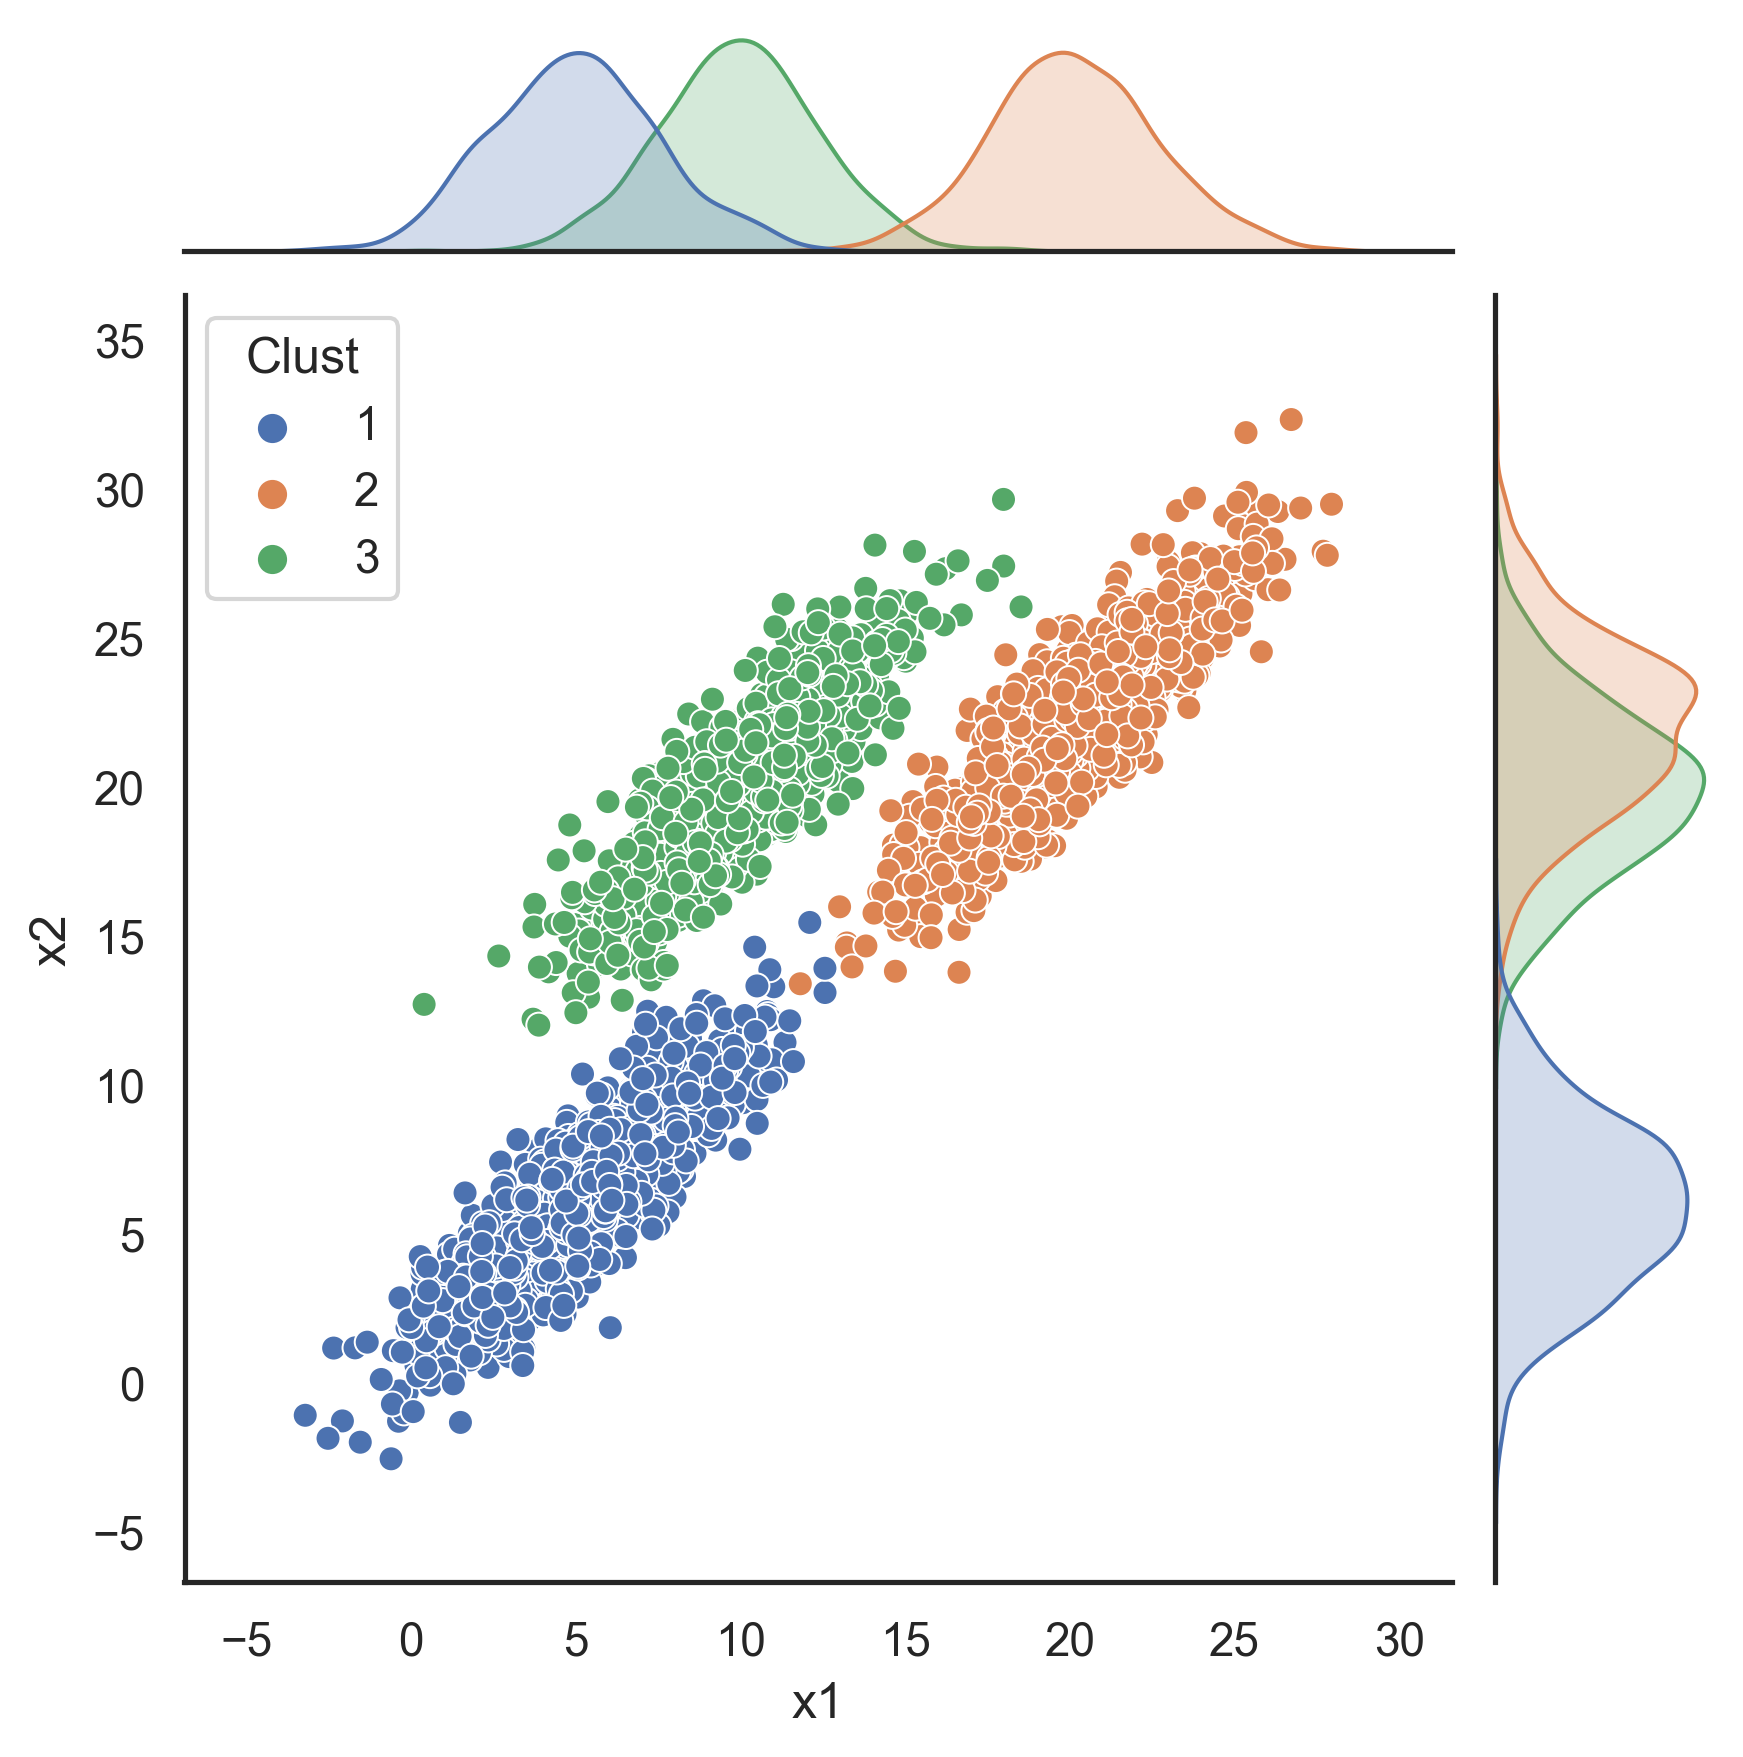
\includegraphics[width=0.45\linewidth]{../Simu_results/sen2.png}
  \caption{Simulation result from equation (17) and its true labels}
  \label{fig:sec}
\end{figure}

Next apply the K-means clustering, spectral clustering and HMM clustering method to the data we just generated, respectively. The cluster results are presented in Figure 2. We can see that the K-means performs the worst because it considers only the Euclidean distance without any parametric assumption. Spectral clustering performs better than K-means clustering but still exist some miss-classifications. HMM outperforms other two algorithm since it assume the emission probability is normally distributed. By doing this, the algorithm will take statistical distance into considerations rather than Euclidean distance.

\begin{figure}[h!]
  \centering
  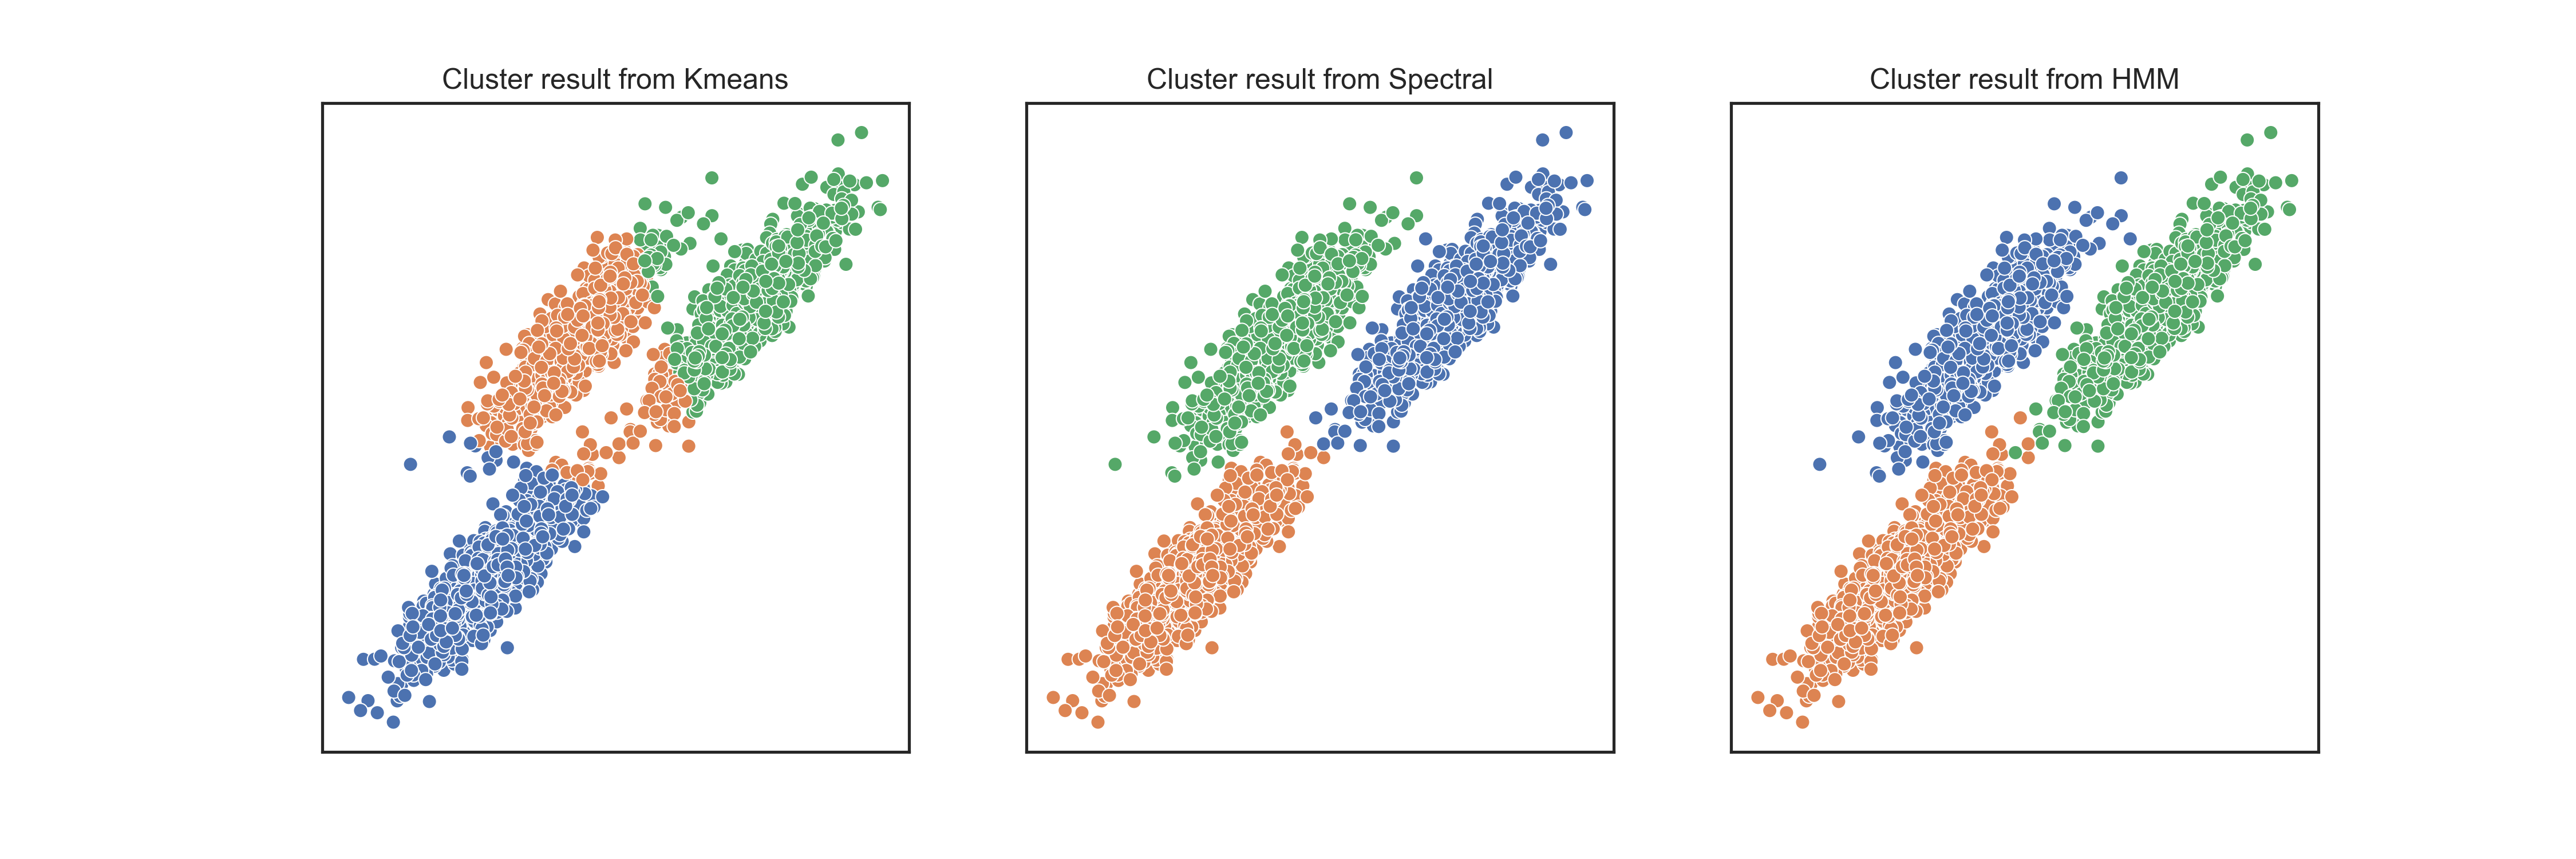
\includegraphics[width=0.8\linewidth]{../Simu_results/sen2_clust.png}
  \caption{Cluster results from K-means Clustering, Spectral Clustering and HMM in scenario 2}
  \label{fig:sec}
\end{figure}

\subsection{Scenario three:  large circle containing a smaller circle}

In the third scenario, consider the following data generating process with two clusters

\begin{equation}
	\boldsymbol{x}_{1i} = 
	\begin{pmatrix}
		x_{11} \\
		x_{21}
	\end{pmatrix}  = 
	\begin{pmatrix}
		z_{11} \\
		z_{21}
	\end{pmatrix} + 
	\begin{pmatrix}
		\epsilon_{11} \\
		\epsilon_{21}
	\end{pmatrix}
	 \quad s.t. \quad 
	z_{11}^2 + z_{12}^2 = 1 \mbox{ and }
	\epsilon_{11}, \epsilon_{21} \sim_{iid} N(0, \sigma^2), \quad i = 1,..,n
\end{equation}

\begin{equation} 
	\boldsymbol{x}_{2i} = 
	\begin{pmatrix}
		x_{12} \\
		x_{22}
	\end{pmatrix}  = 
	\begin{pmatrix}
		z_{12} \\
		z_{22}
	\end{pmatrix} + 
	\begin{pmatrix}
		\epsilon_{12} \\
		\epsilon_{22}
	\end{pmatrix}
	 \quad s.t. \quad 
	z_{21}^2 + z_{22}^2 = \frac{1}{2} \mbox{ and }
	\epsilon_{12}, \epsilon_{22} \sim_{iid} N(0, \sigma^2), \quad i = 1,...,n
\end{equation}

I use the \texttt{make\_circles()} function with $\sigma^2 = 0.08$ in sklearn module to generate the data from equation (18) and (19). The simulations from the DGP in equation (18) and (19) is presented in Figure 4.

\

\begin{figure}[h!]
  \centering
  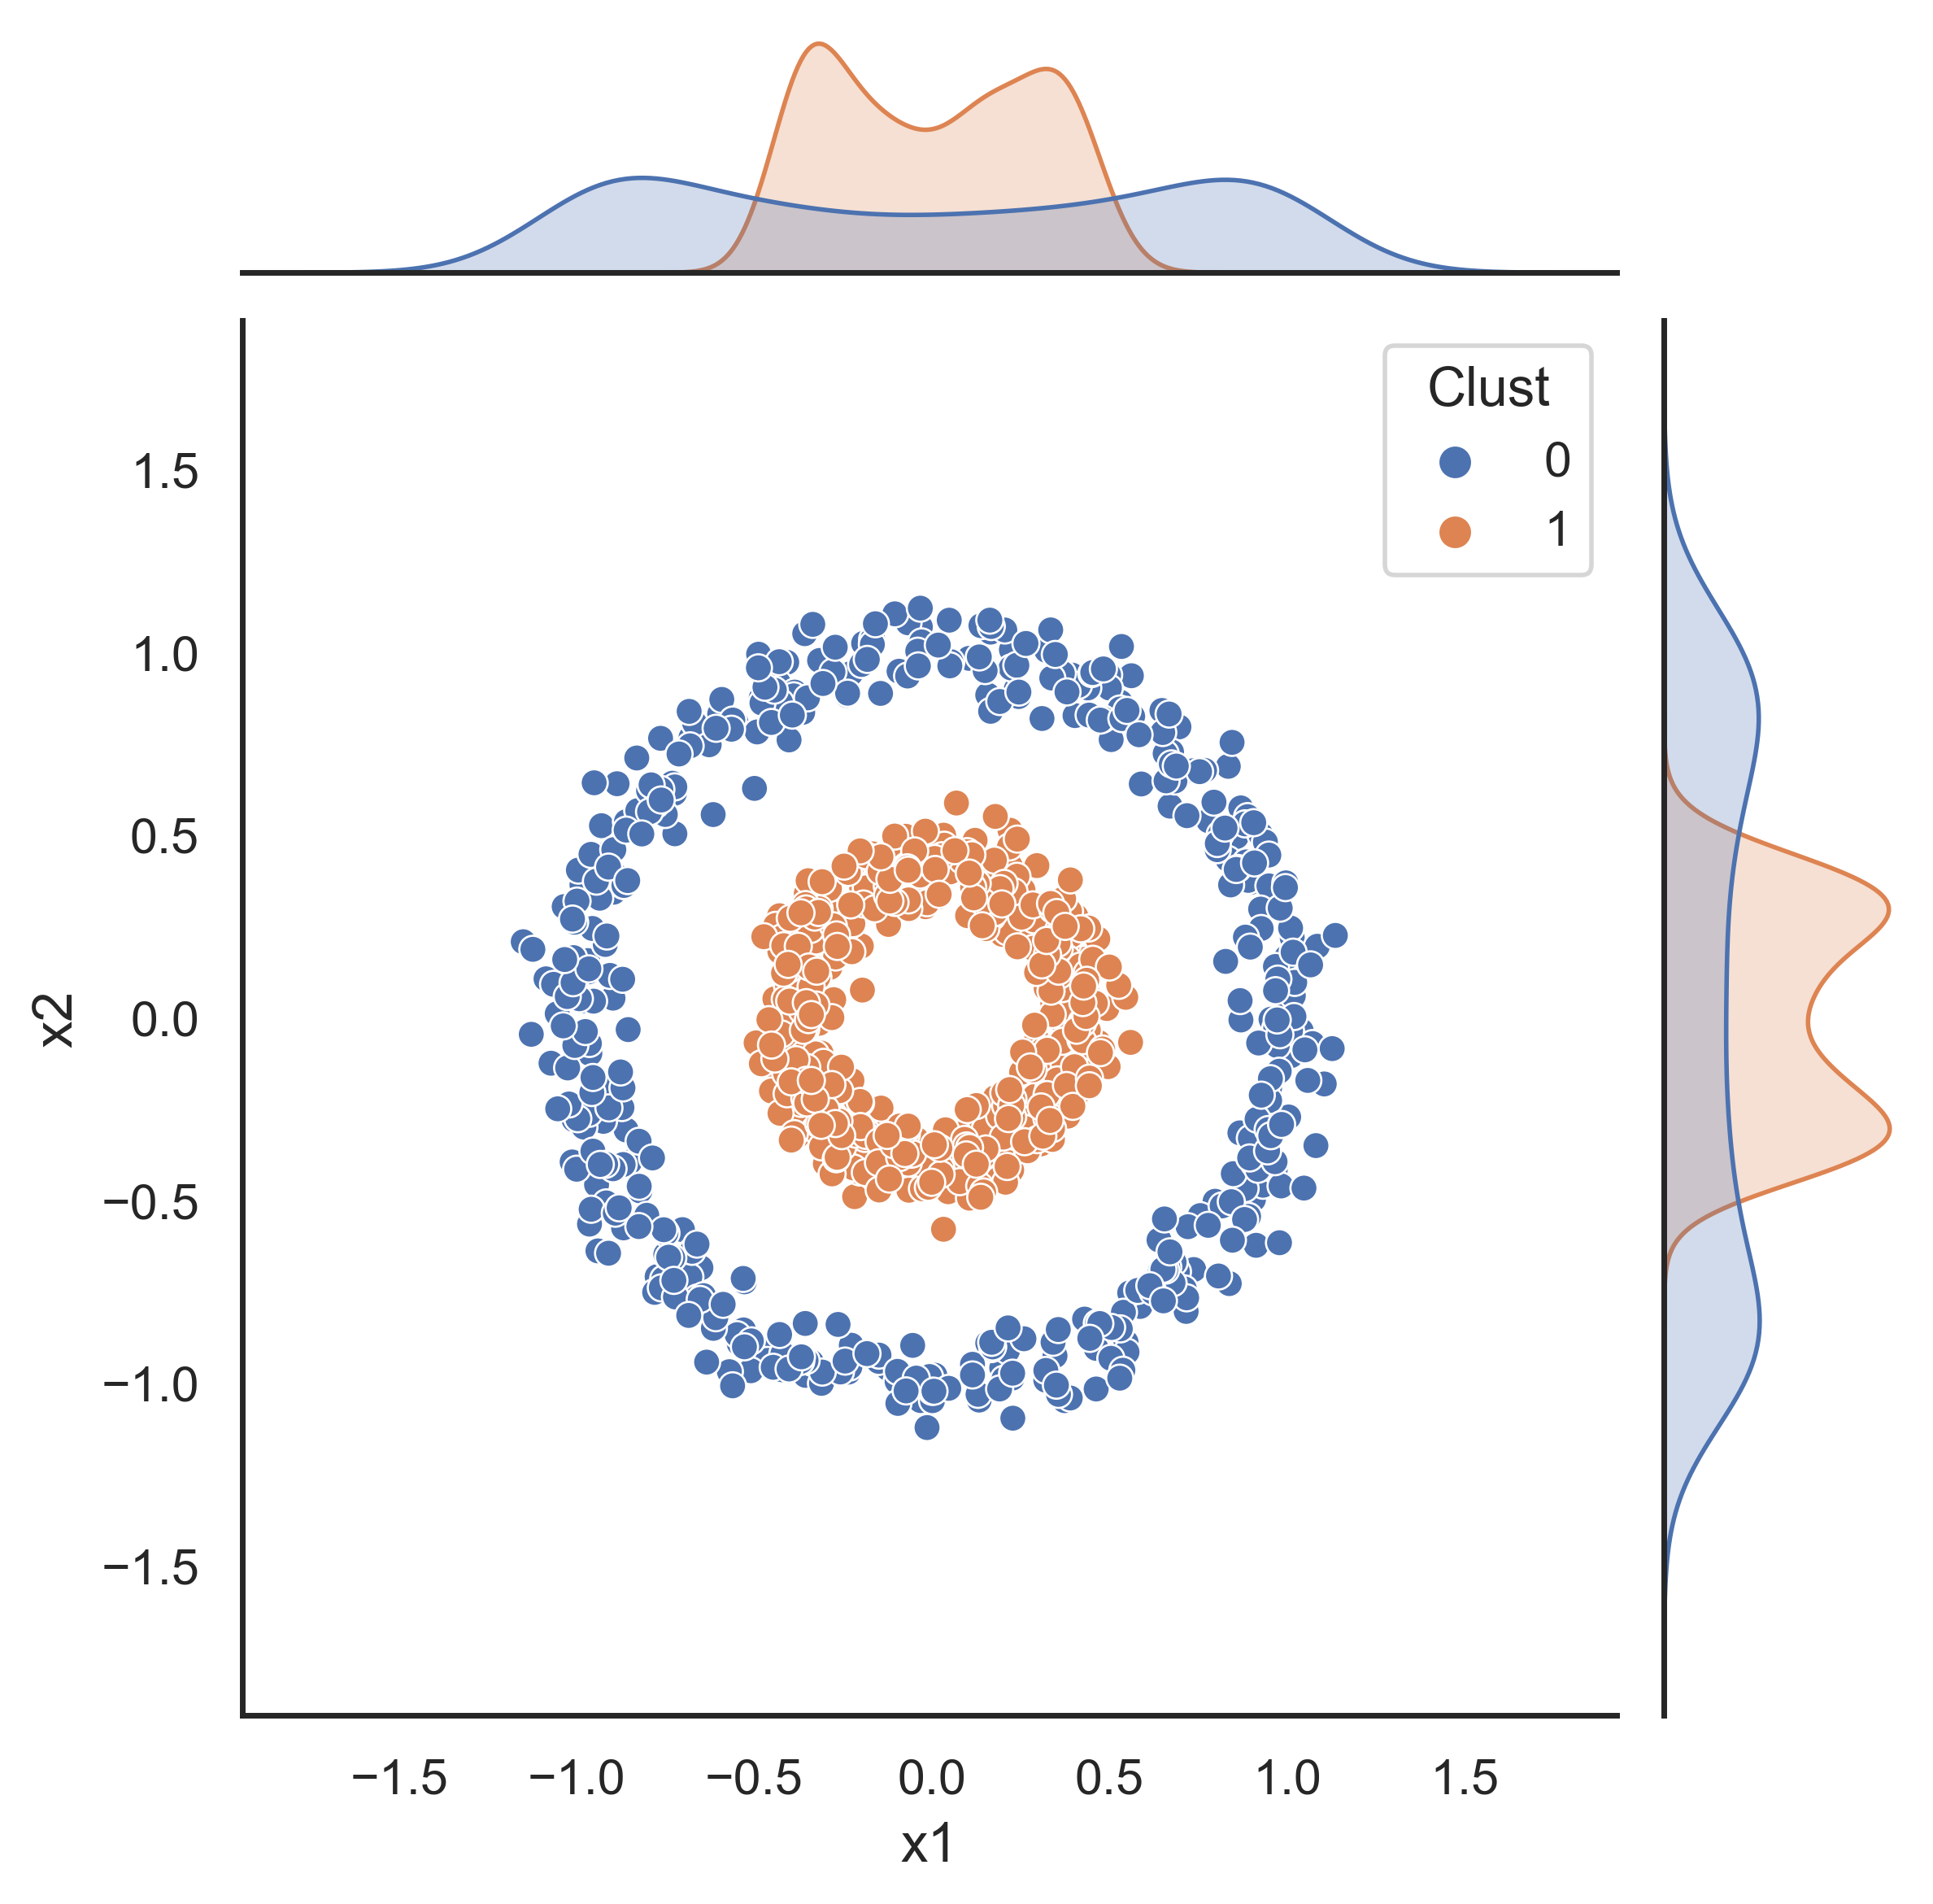
\includegraphics[width=0.45\linewidth]{../Simu_results/sen3.png}
  \caption{Simulation result from equation (18) and (19), and its true labels}
  \label{fig:sec}
\end{figure}

Next apply the K-means clustering, spectral clustering and HMM clustering method to the data we just generated, respectively. The K-means clustering and HMM clustering algorithm performs poorly at both around 50\% accuracy rate. The reason is that these two algorithm essentially one of board approach called compactness. K-means defines closeness as Euclidean distance in most situations, and HMM defines closeness as statistical distance via probability assumption and EM algorithm. On the other hand, spectral clustering is another board approach called connectivity. Even if the distance between each point is ver small, if they are not connected in the graph build from the data, they are not clustered together.


\begin{figure}[h!]
  \centering
  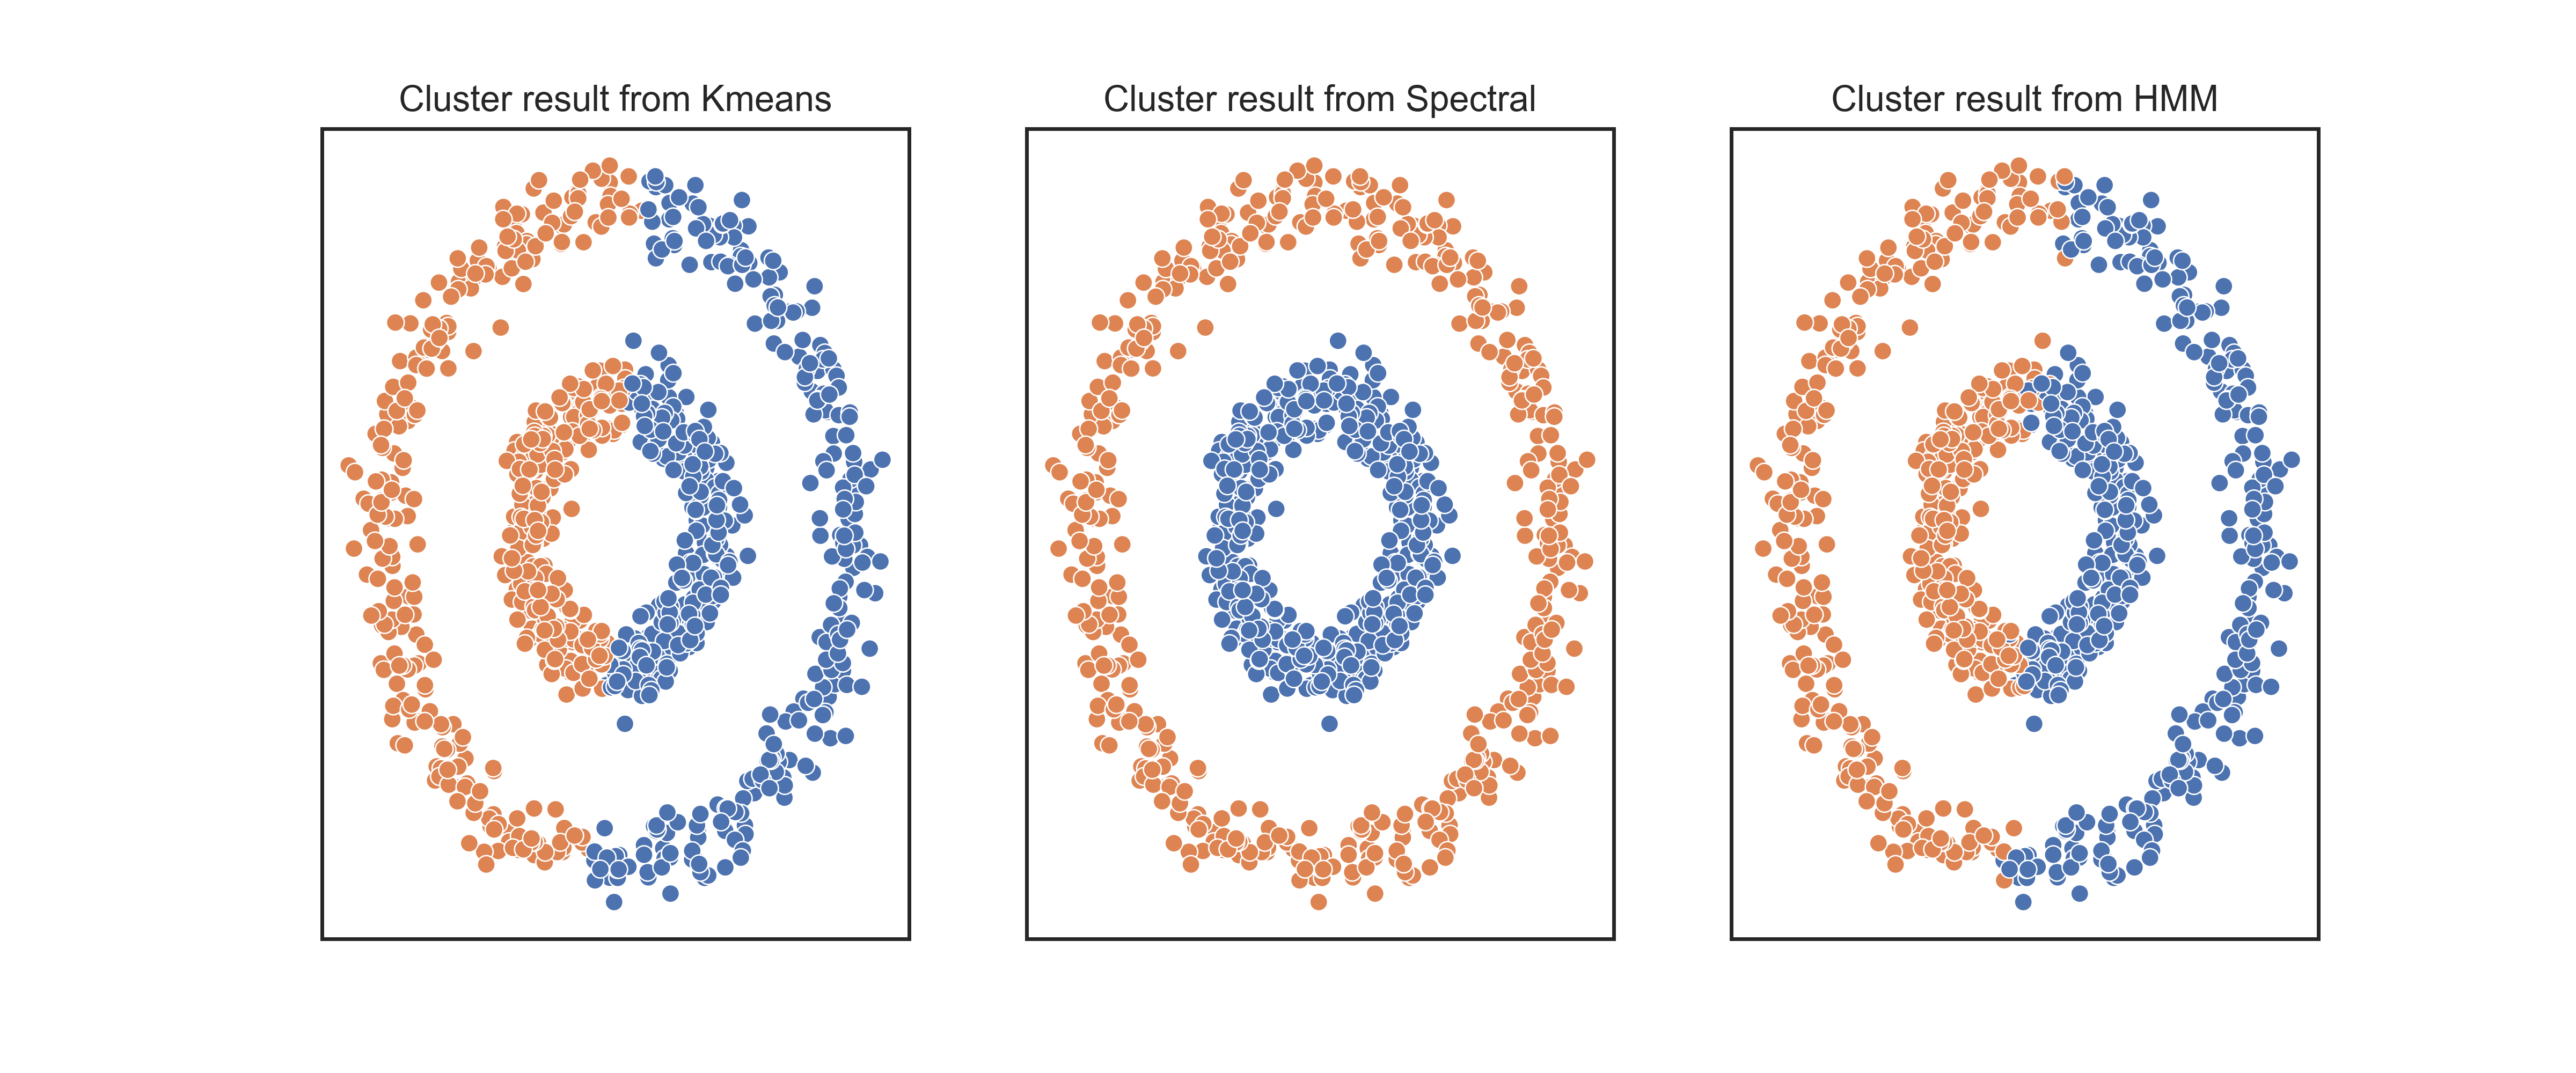
\includegraphics[width=0.8\linewidth]{../Simu_results/sen3_clust.png}
  \caption{Cluster results from K-means Clustering, Spectral Clustering and HMM in scenario 3}
\end{figure}

\section{Practical Example}

I've divided this section into two parts. I am going to start with the applications in area of image compression, particularly in \textit{vector quantization} or \textit{color quantization}. Next, utilizing the image segmentation techniques to segment a brain tumor based on magnetic resonance imaging (MRI).

\subsection{Color Quantization}

The K-means clustering algorithm is a commonly used technique to achieve color quantization in digital image processing. It is a process that reduces the number of distinct colors used in an image, i.e. the number of combination of values in each pixel with RGB-color space. The left image in Figure 7 is a digitized photograph of \textit{London Bridge}. It consists 1200 x 1200 pixels, where each pixel is RGB-scale value ranging from 0 to 255 in 3-dimensional space, and hence requires 32 bits of storage per pixel. Therefore, this image needs 4 Megabyte for the storage. The remaining images in Figure 7 are VQ-compressed version of original image obtain from K-means, which $K$ equals to 64 and 10, respectively. These images require much less storage space but at some loss in quality, and the loss is severer as the K parameter decreasing.

\begin{figure}[h!]%
    \centering
    \subfloat{{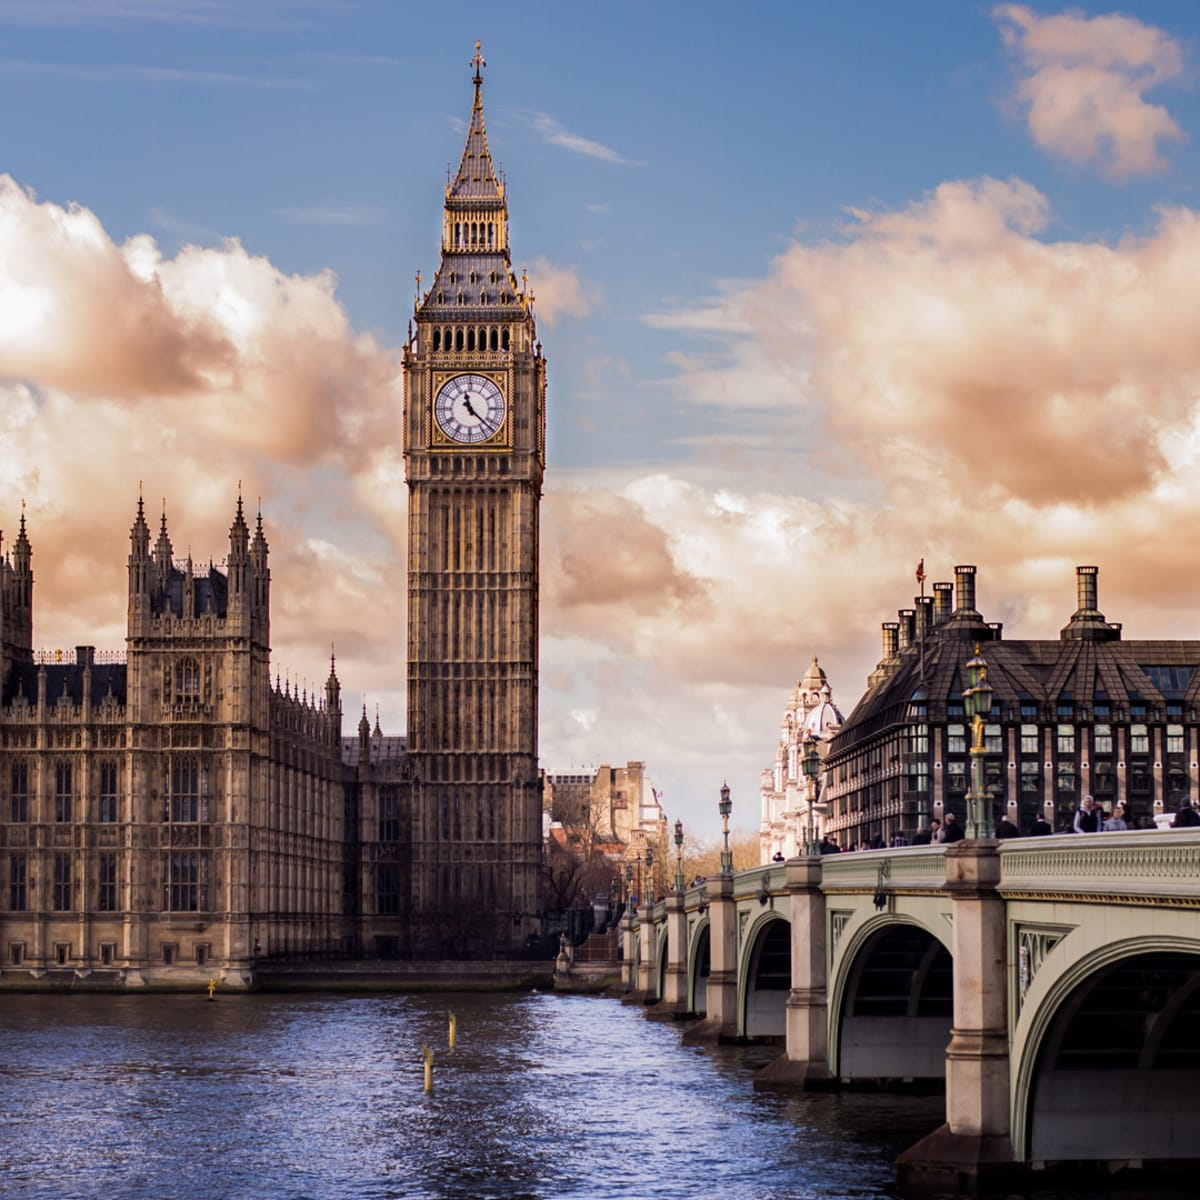
\includegraphics[width=0.3\textwidth]{../Cluster_results/London/London.png}}}%
    \subfloat{{\includegraphics[width=0.3\textwidth]{../Cluster_results/London/London_kmeans_64.png}}}
    \subfloat{{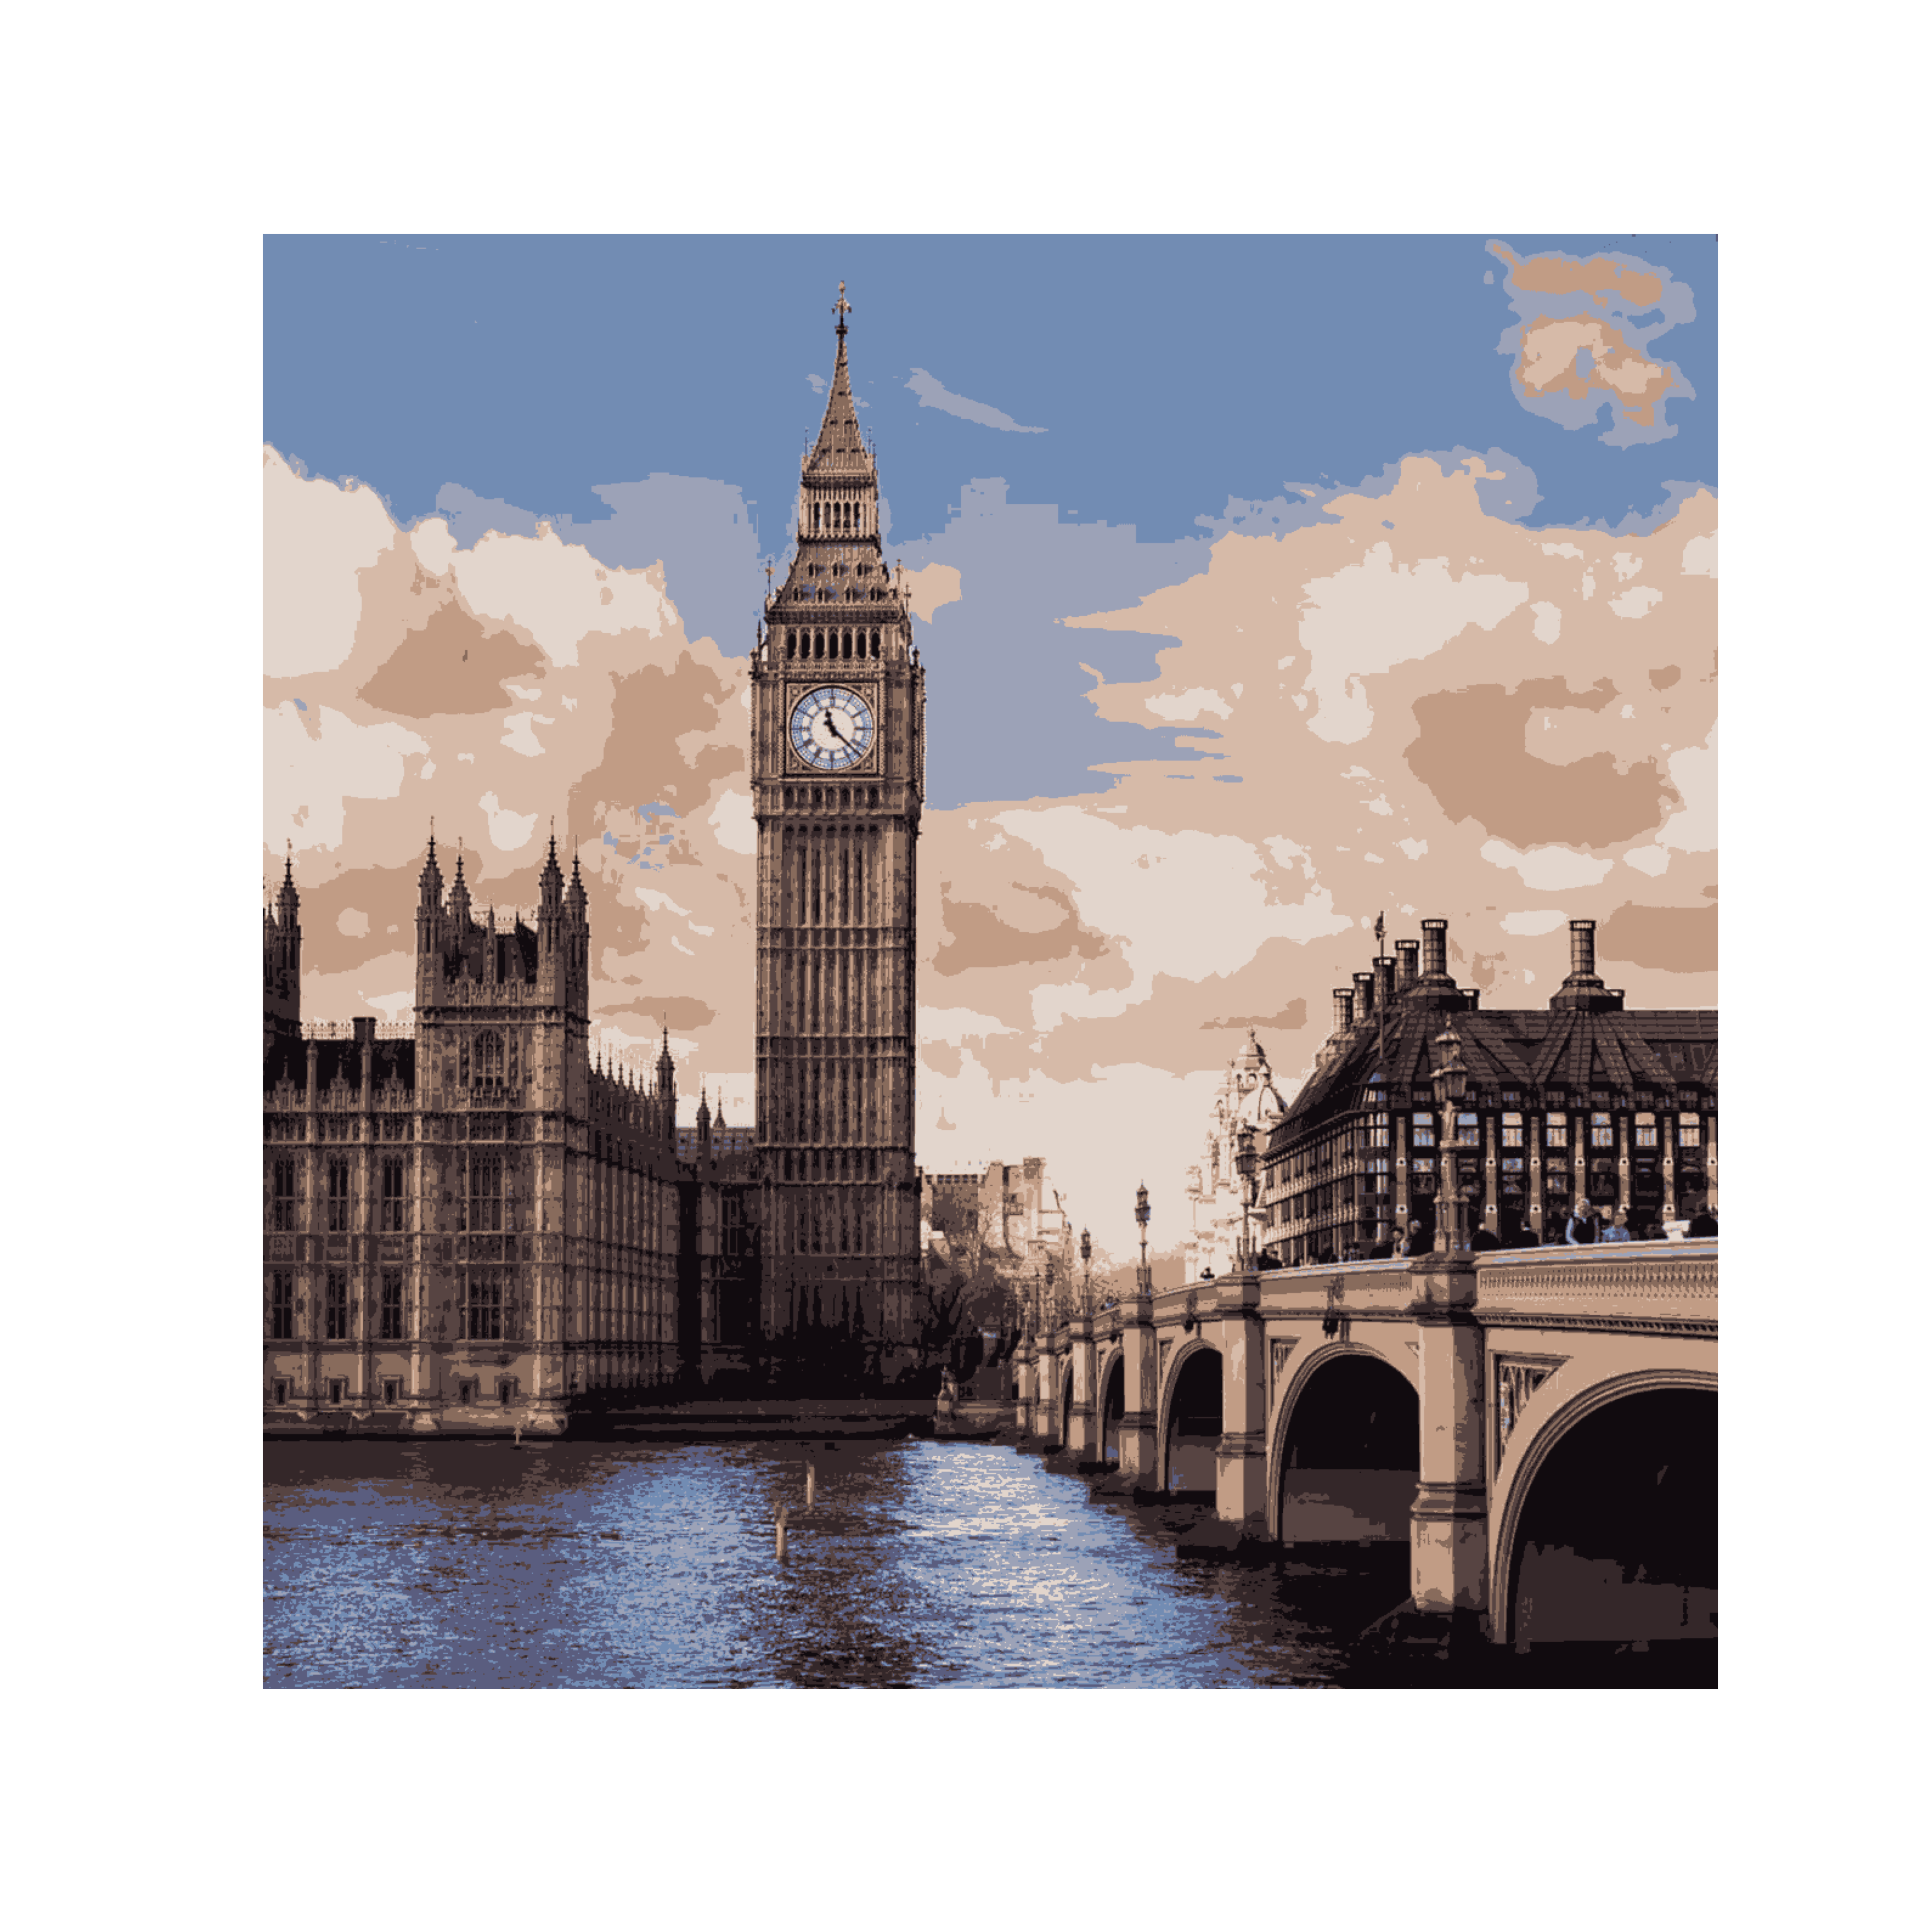
\includegraphics[width=0.3\textwidth]{../Cluster_results/London/London_kmeans_10.png}}}
    \caption{\textit{London Bridge in London, UK}. The left panel is original image. The middle panel is the compressed image using 64 code vectors (64 clusters in K-means). The right panel is the compressed image using 5 code vectors (5 clusters in K-means)}.
\end{figure}

I demonstrate another example of color quantization in Figure 8. The left image in Figure 8 is photograph of three \textit{cute Shiba}. It consists 533 x 800 pixels in RGB-color space. The remaining images in Figure 8 are VQ-compressed version of original image obtained from K-means either, which $K$ equals to 64 and 10, respectively.

\begin{figure}[h!]%
    \centering
    \subfloat{{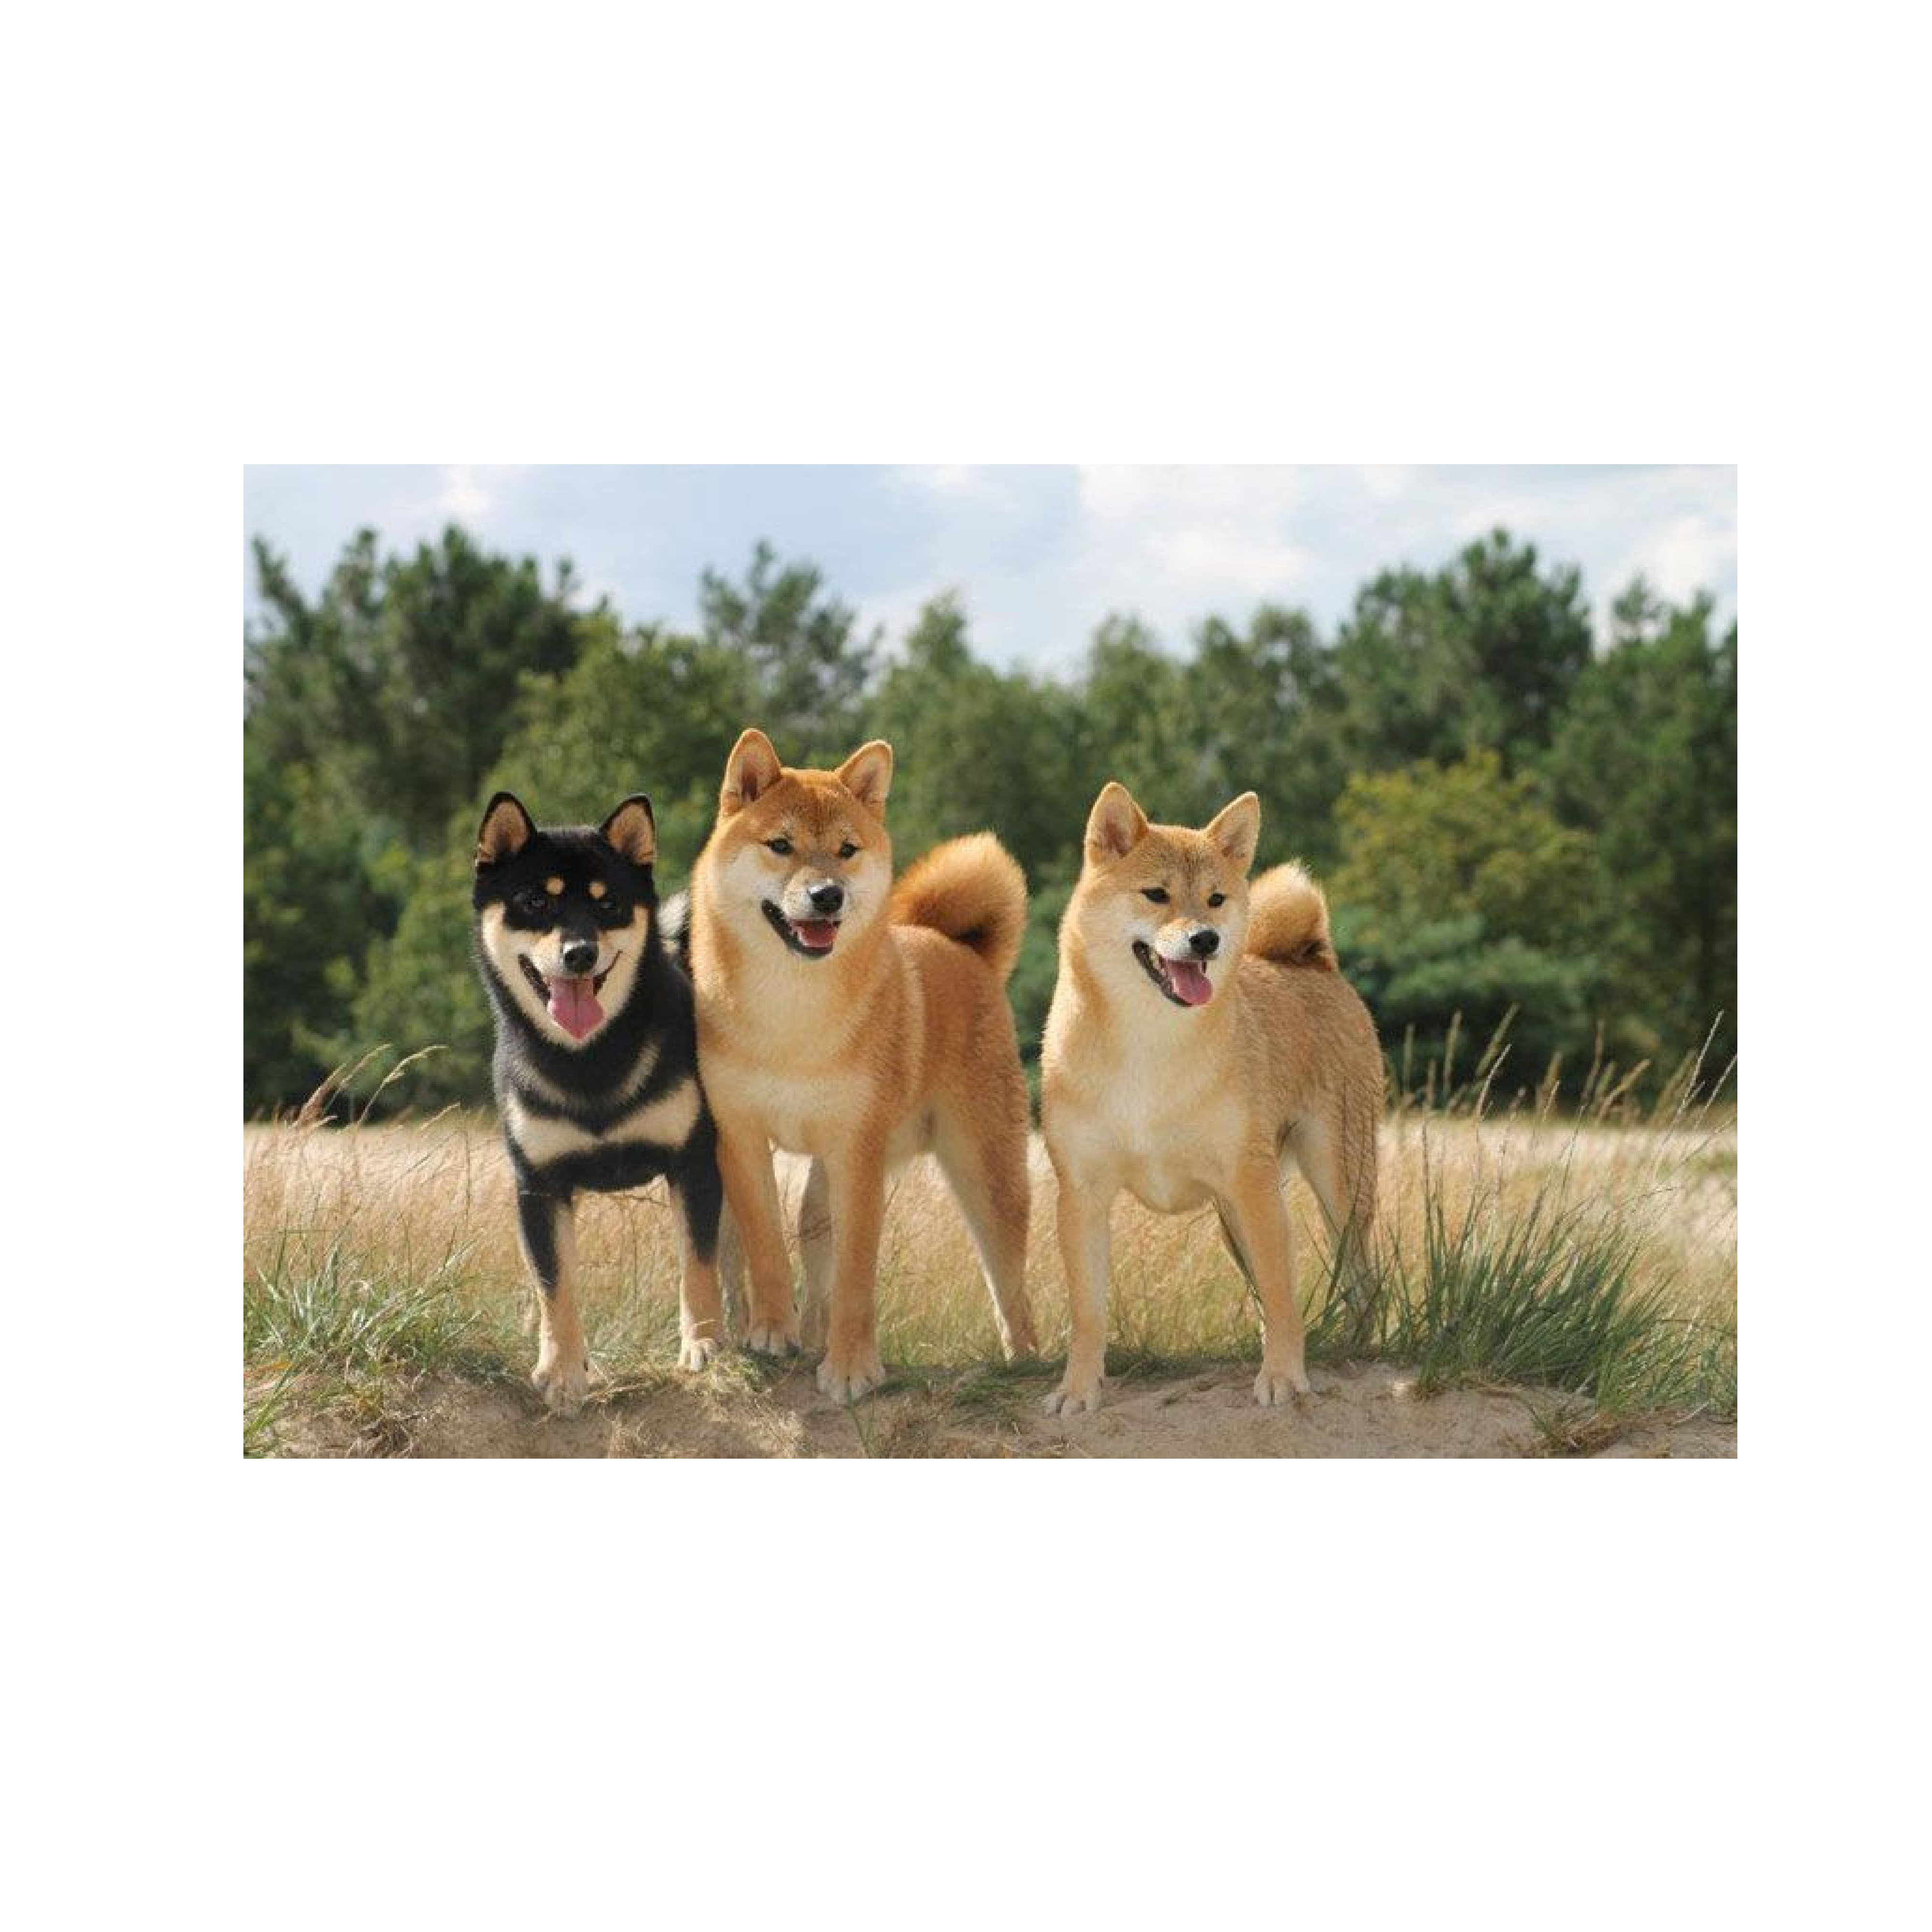
\includegraphics[width=0.3\textwidth]{../Cluster_results/Shiba/Shiba.png}}}%
    \subfloat{{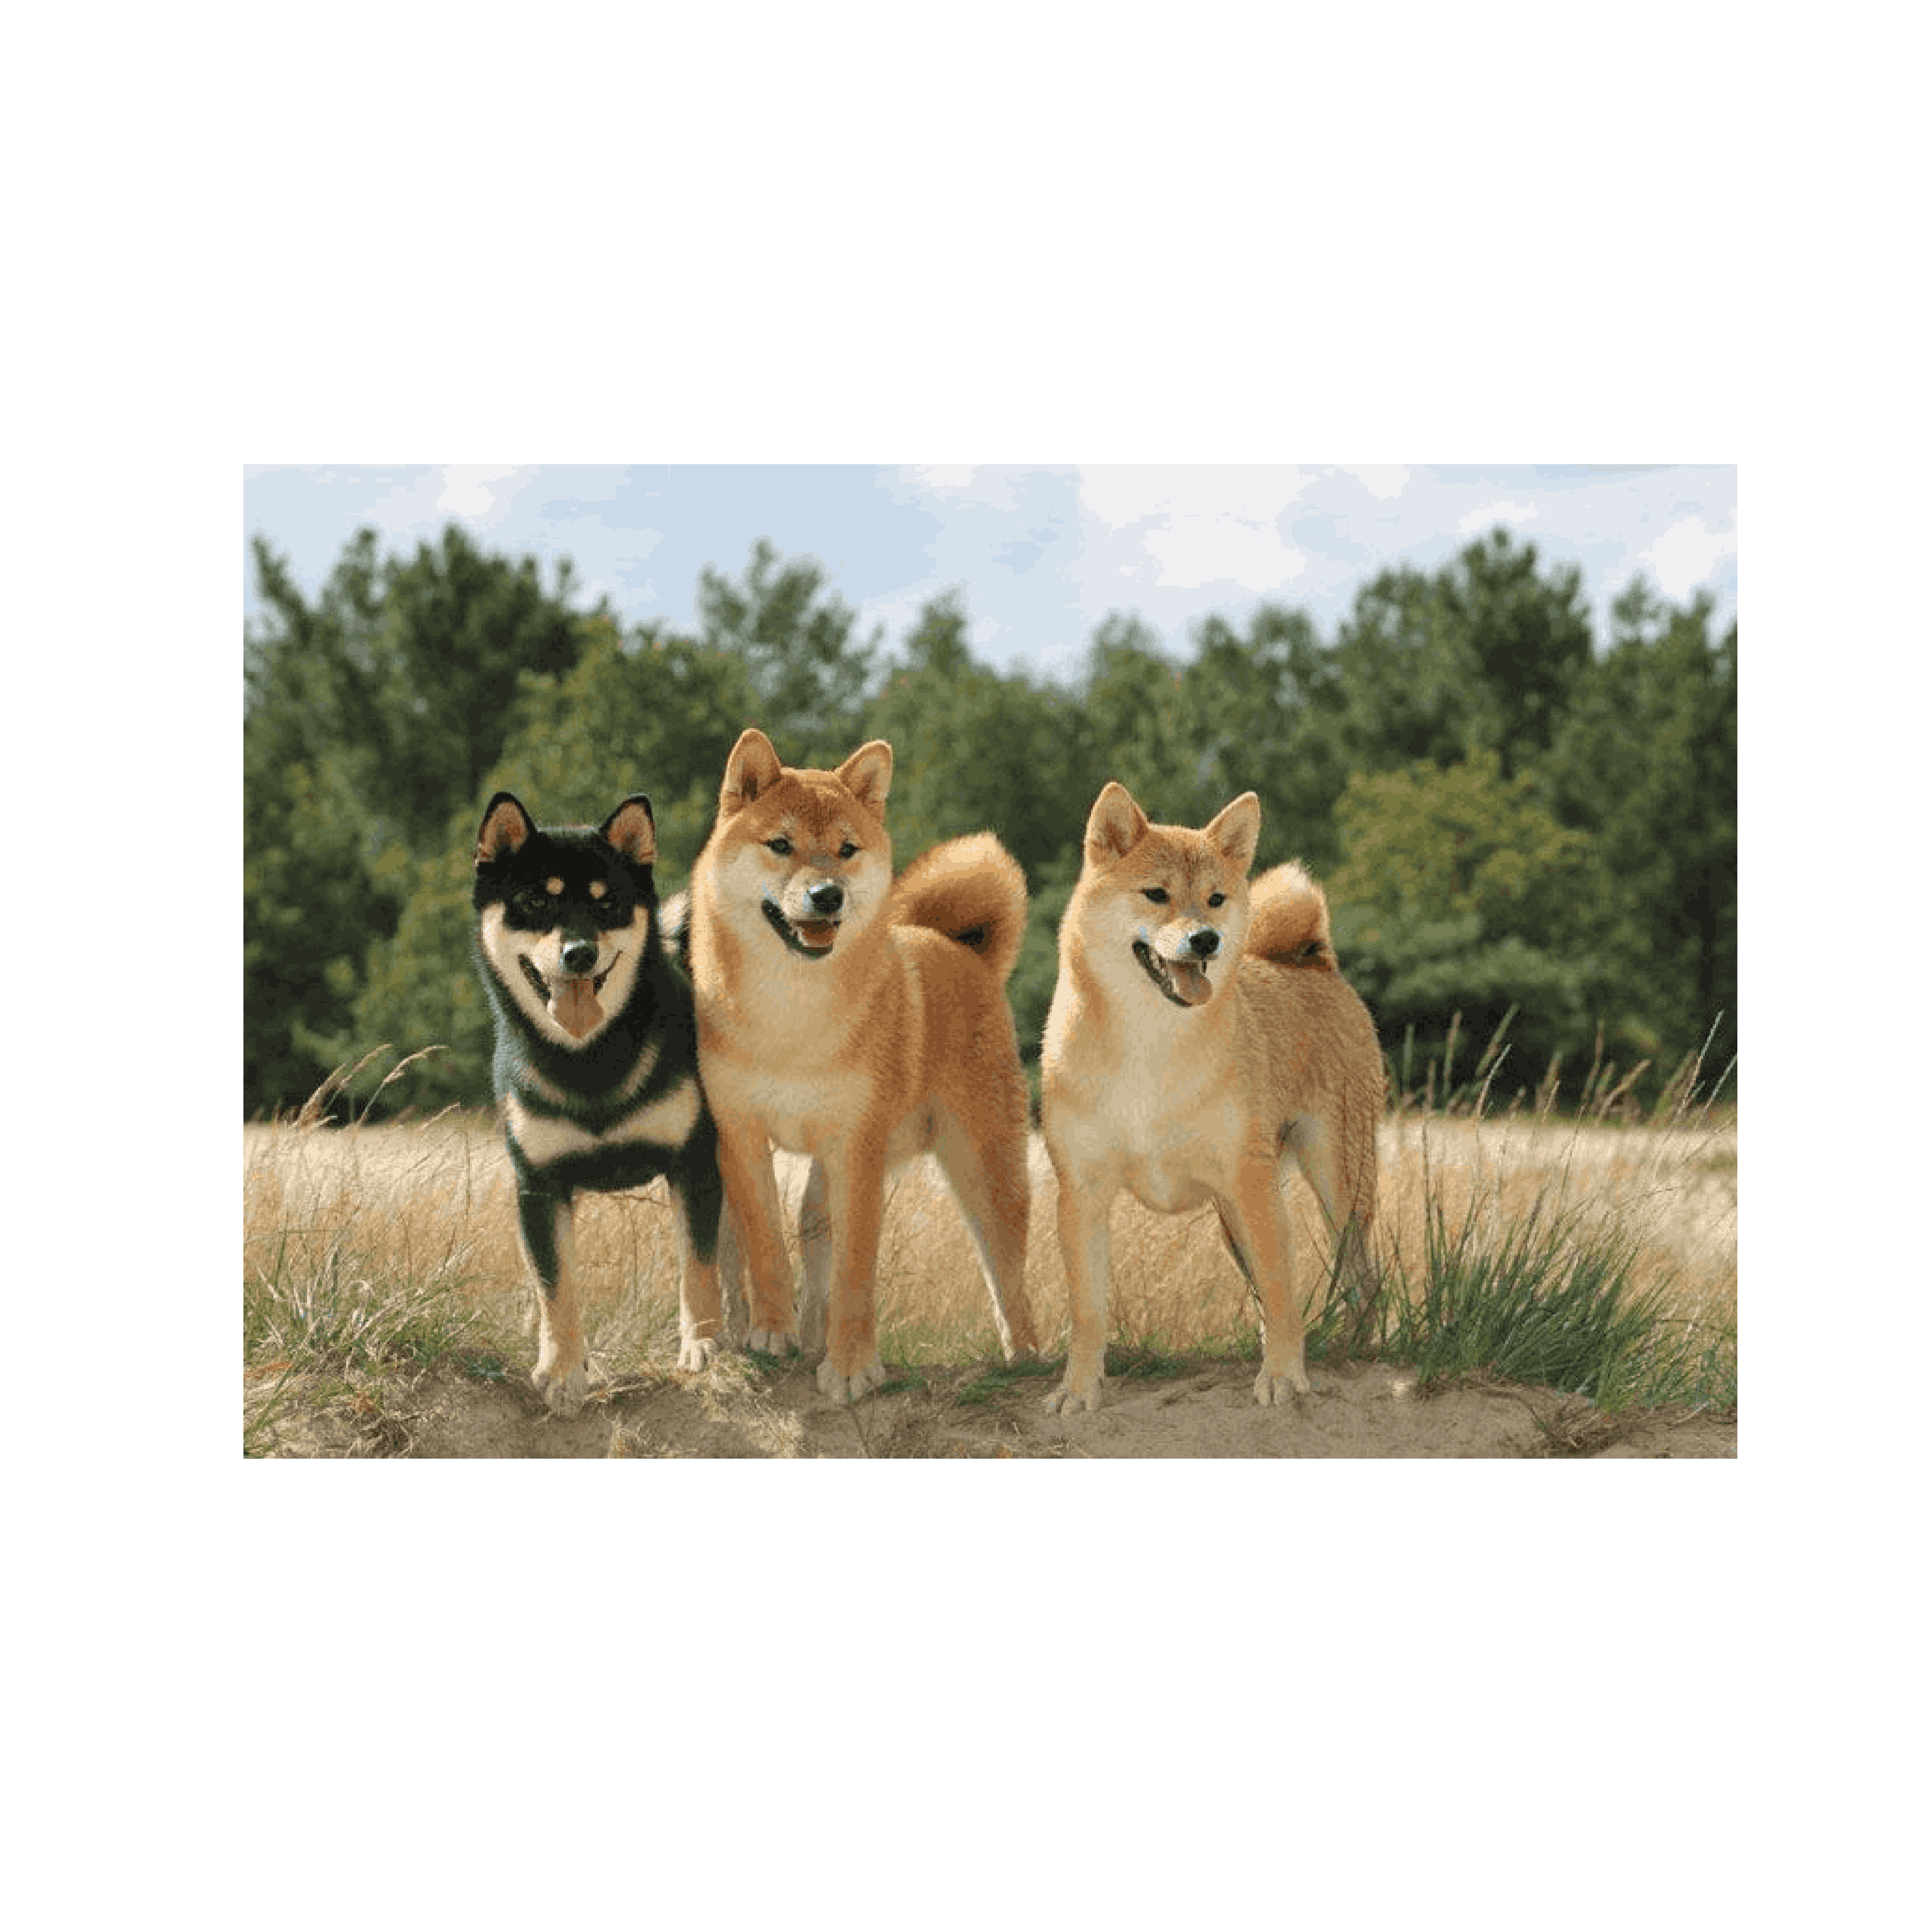
\includegraphics[width=0.3\textwidth]{../Cluster_results/Shiba/Shiba_kmeans_64.png}}}
    \subfloat{{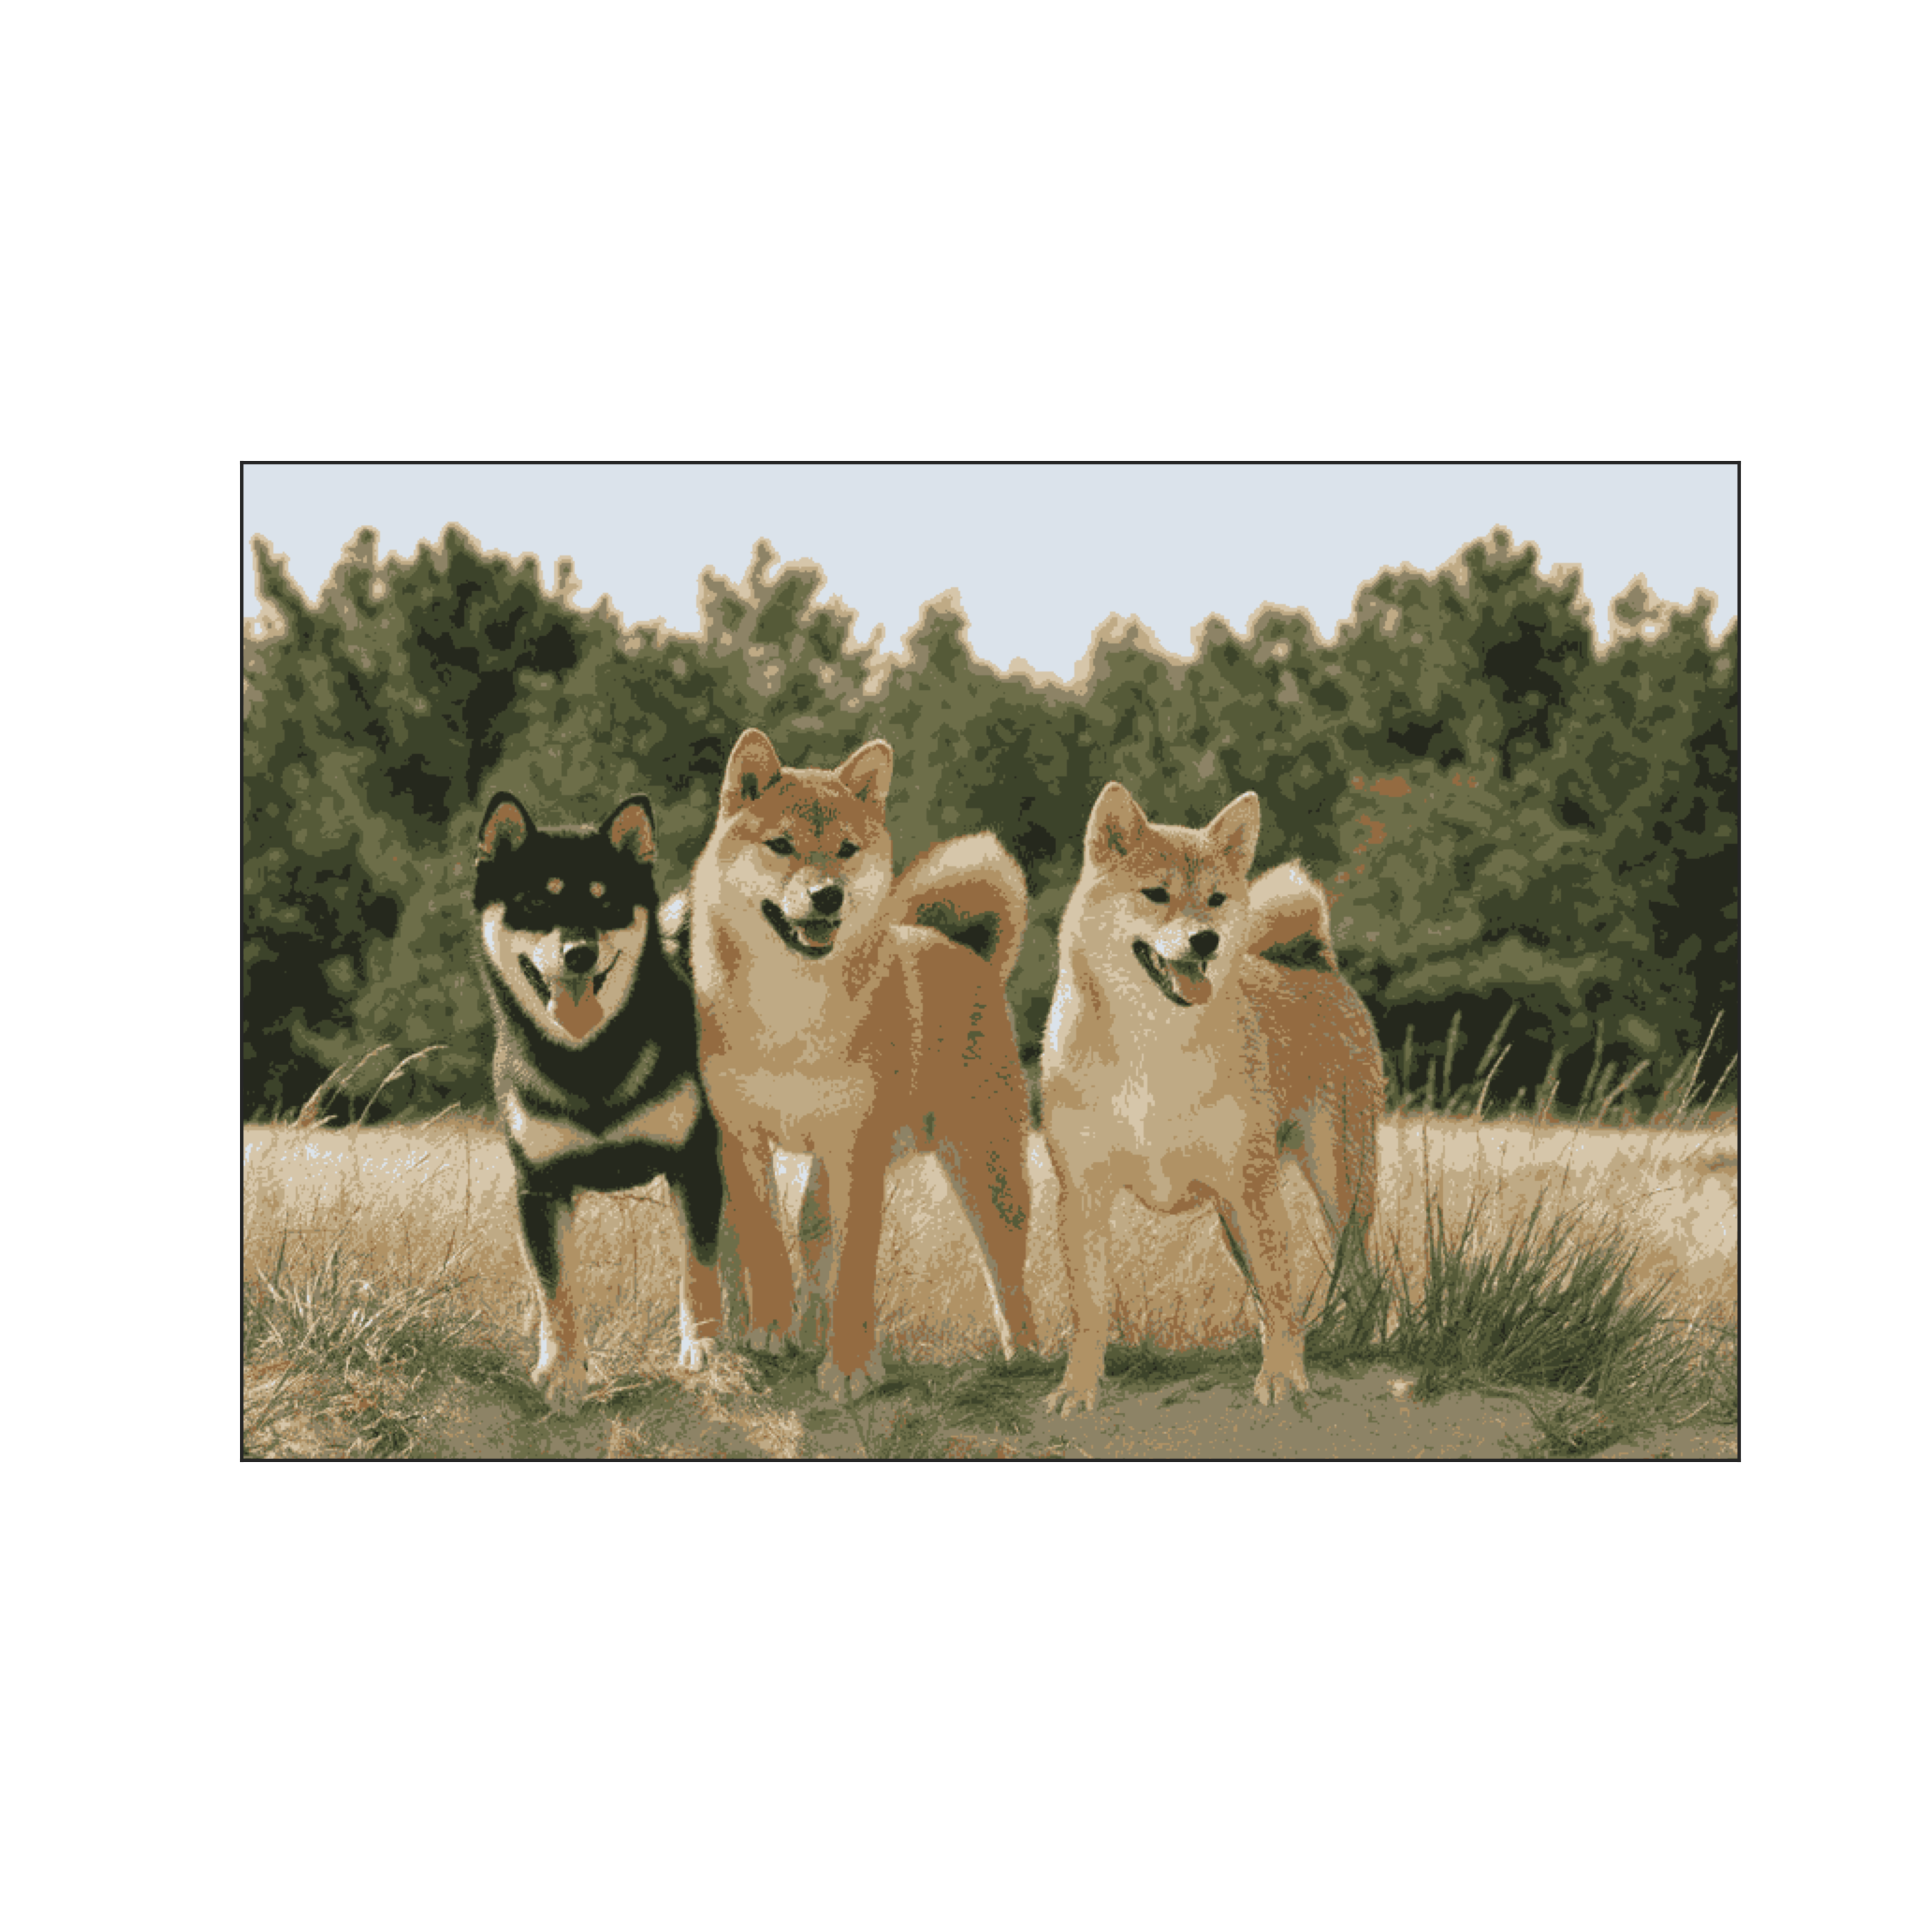
\includegraphics[width=0.3\textwidth]{../Cluster_results/Shiba/Shiba_kmeans_10.png}}}
    \caption{\textit{three cute Shiba being happy on the grass}. The left panel is original image. The middle panel is the compressed image using 64 code vectors (64 clusters in K-means). The right panel is the compressed image using 5 code vectors (5 clusters in K-means).}
\end{figure}


\subsection{Medical Image Segmentation}

Medical image segmentation is a task of automatically segmenting the targets of interest in a medical image, such as X-ray or magnetic resonance images. It has an essential role in computer-aided diagnosis system. Specifically, I will segment brain tumor from MRI in this section. A brain tumor is a mass of abnormally growing cells in the brain or skull. MRI  provide a detained image of the brain, and it is one of the most common tests used to diagnose brain tumors. Brain tumor segmentation from MR image can have great impact for the improvement of diagnostics, growth rate prediction and treatment planning. U-Net is a NN-based method to perform image segmentation, and it outperforms the other techniques in most situation, especially in medical imaging problem.  Due to the constraint of topics and time allowed for this midterm project, I only use techniques introduced in section 2 to perform the segmentation task: K-means clustering, spectral clustering and HMM.

\

The brain tumor image is presented in Figure 9, which is obtained from Stanford brain tumor center. There is a obvious white block of tumor in this MRI. Next, I perform $K=5$ clusters image segmentation using K-means clustering, spectral clustering and HMM with the following settings, respectively, as a demonstration to show the clustering results from these methods.


\begin{figure}[h!]
  \centering
  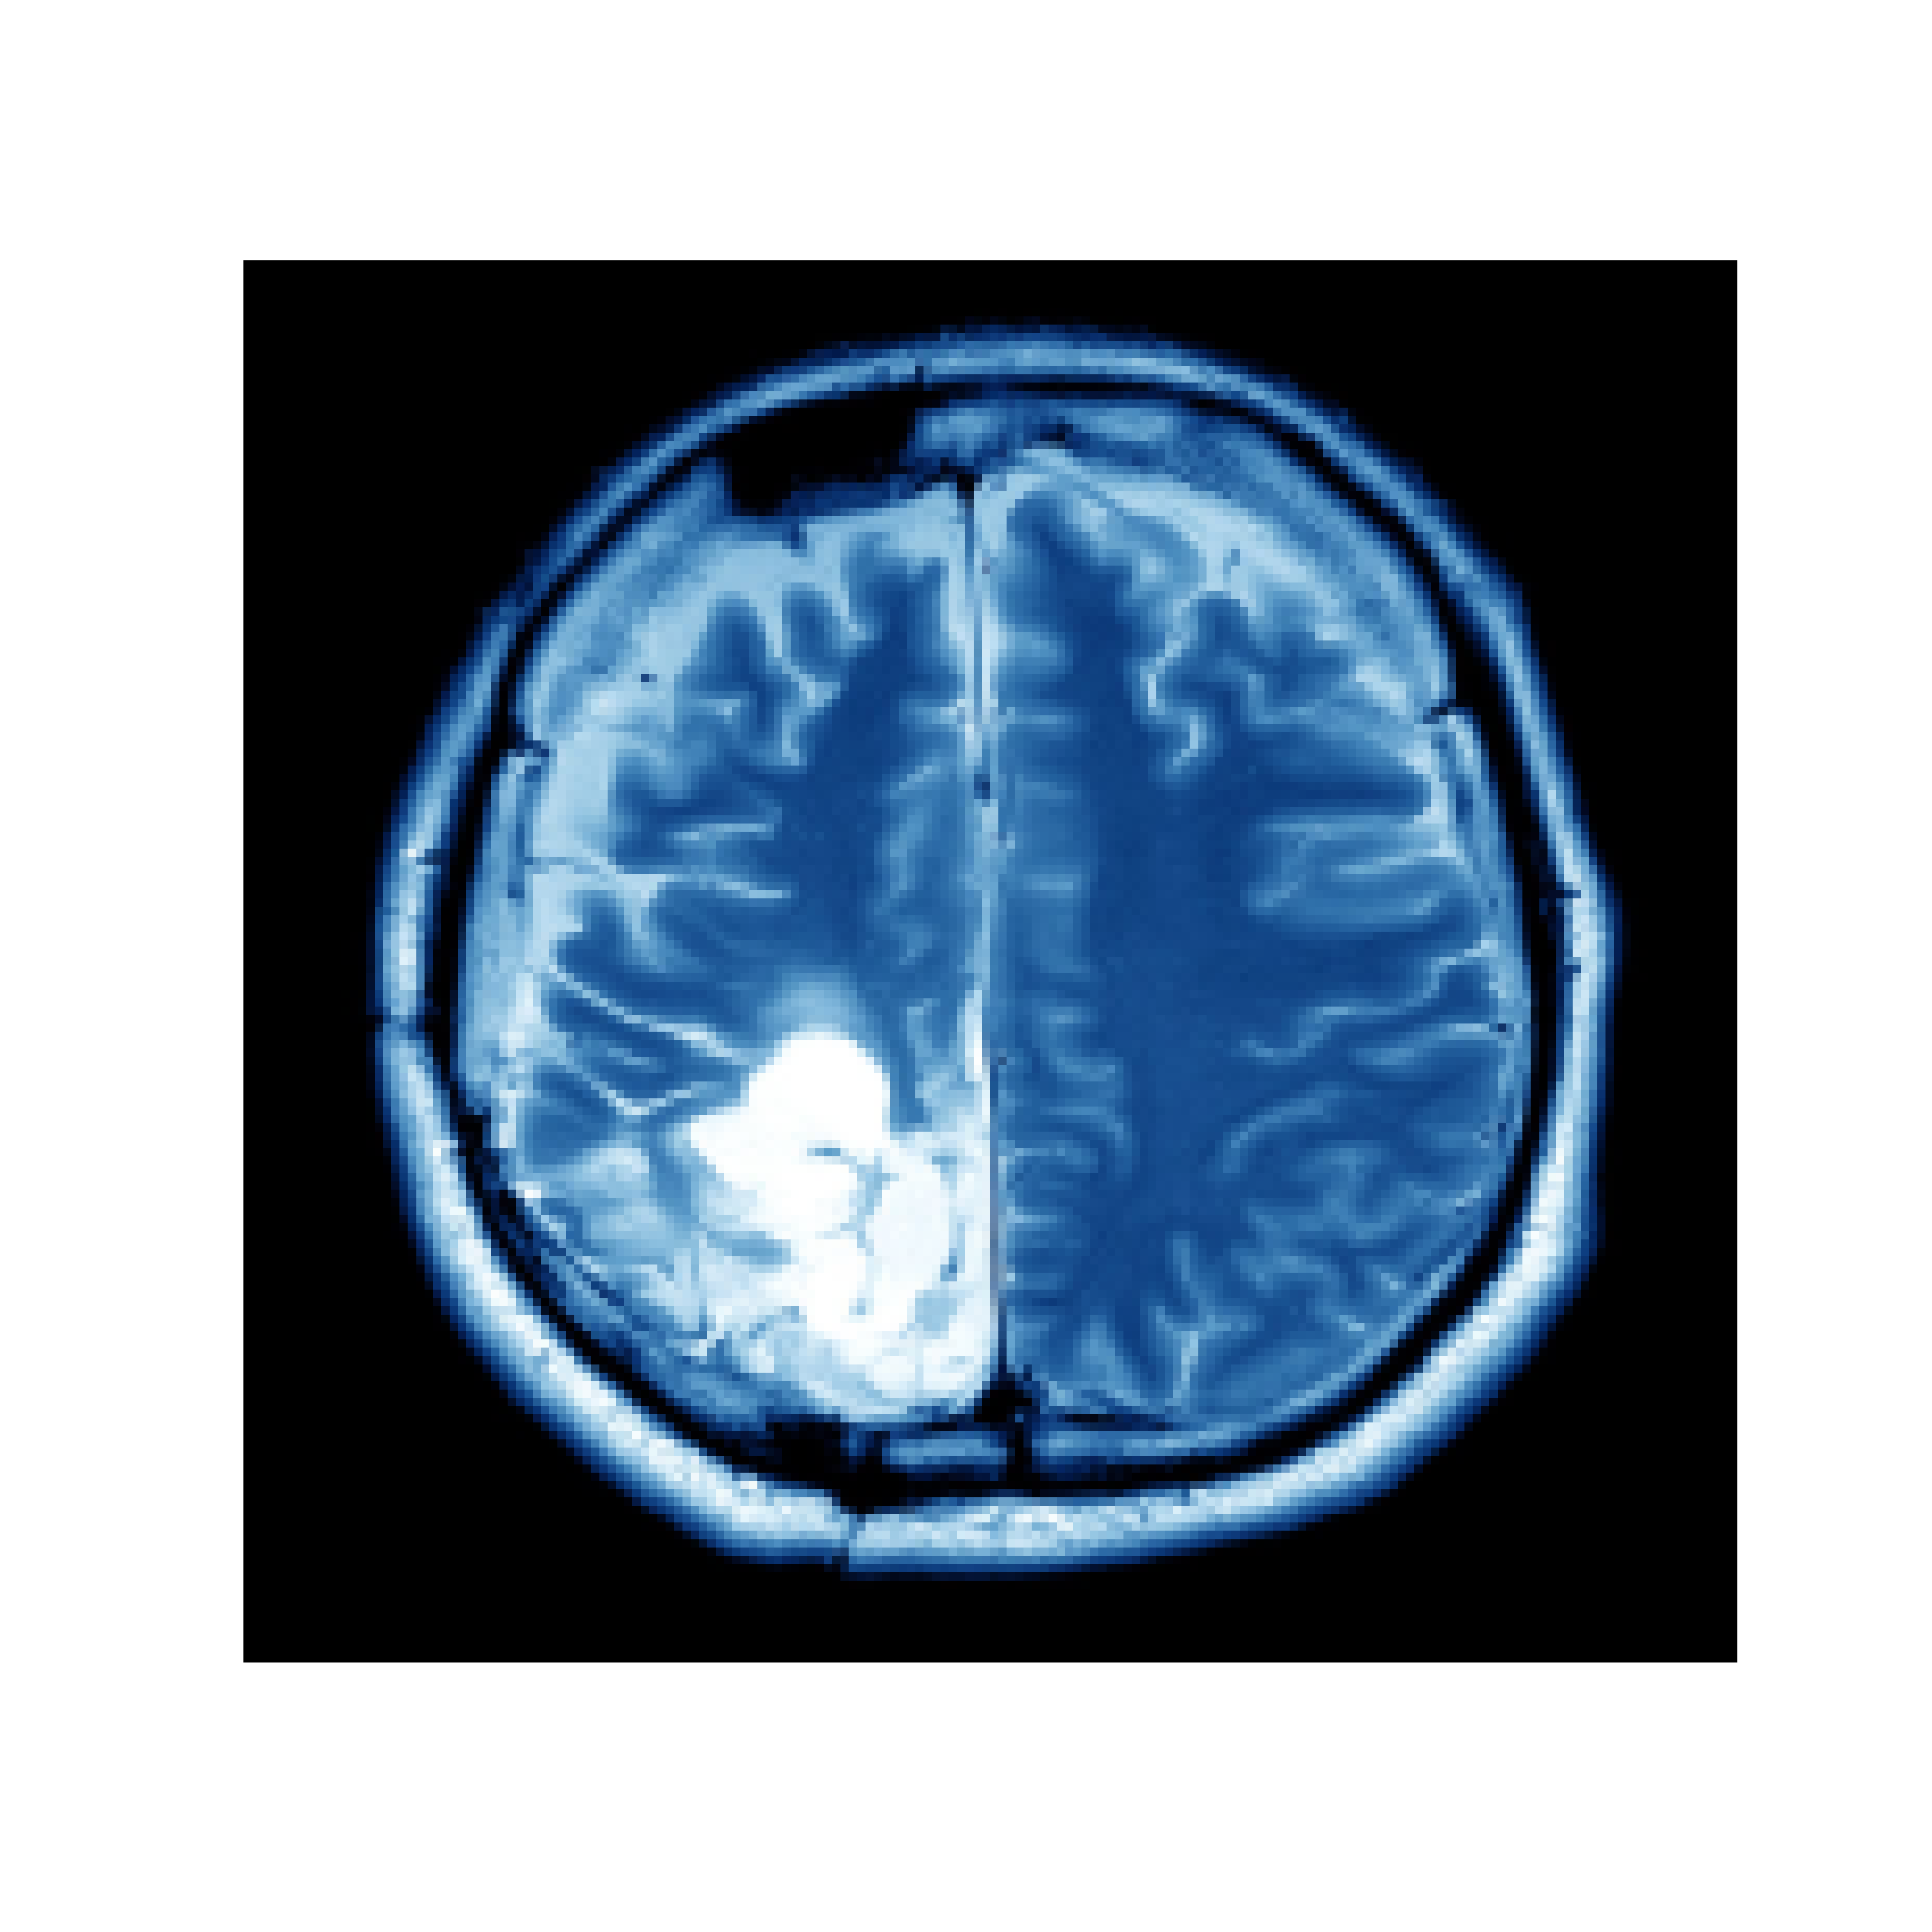
\includegraphics[width=0.4\linewidth]{../Cluster_results/MRI/MRI.png}
  \caption{\textit{tumor brain image} obtained from Stanford brain tumor center}
\end{figure}



\begin{itemize}
	\item K-means clustering algorithm with Forgy method to decide initial set of $k$ means
	\item Spectral clustering algorithm with radial basis weights and k-means to cluster
	\item Hidden Markov Model with normally-distributed emission probabilities
\end{itemize}

The clustering results obtained from these methods are shown in Figure 10. It suggests that the spectral clustering algorithm successfully segment the area of brain tumor in the MRI, while k-means clustering and HMM performs poorly at segmenting the tumor. Next, I further draw a border based on the clustering results obtained from spectral clustering, which is shown in Figure 12. It shows that spectral clustering algorithm can segment the tumor precisely.

\begin{figure}[h!]%
    \centering
    \subfloat{{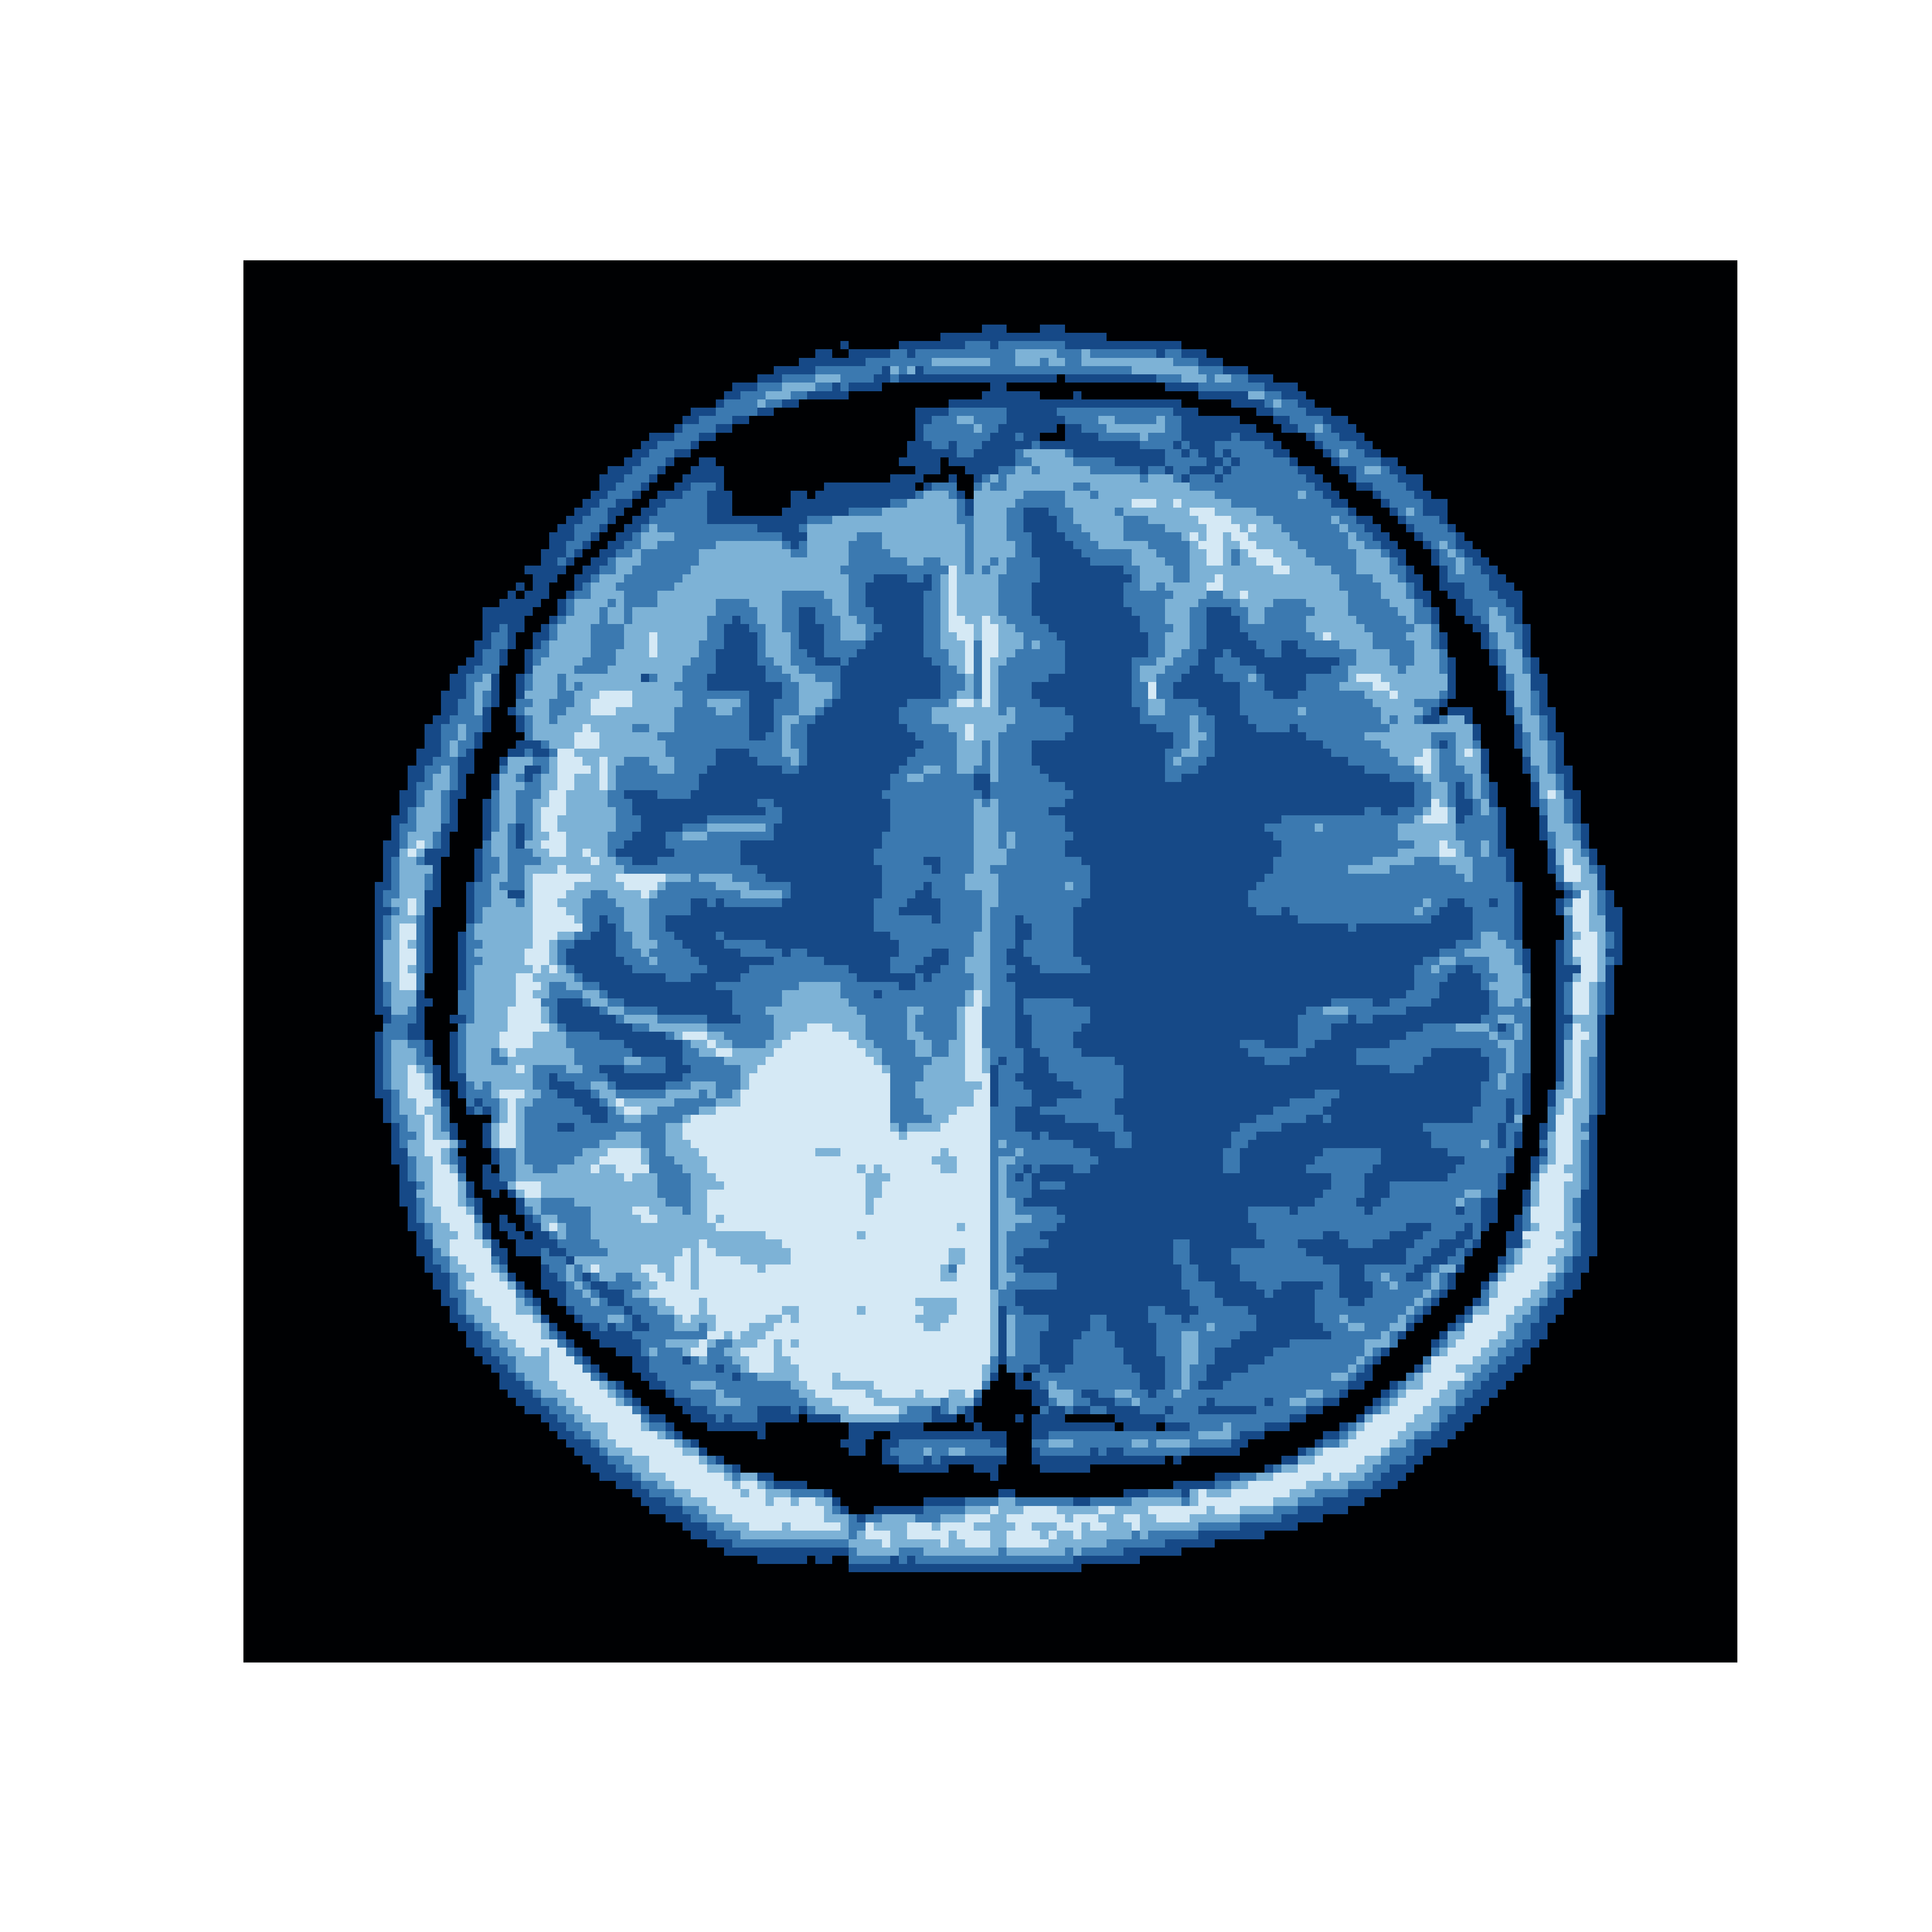
\includegraphics[width=0.3\textwidth]{../Cluster_results/MRI/MRI_kmeans.png}}}%
    \subfloat{{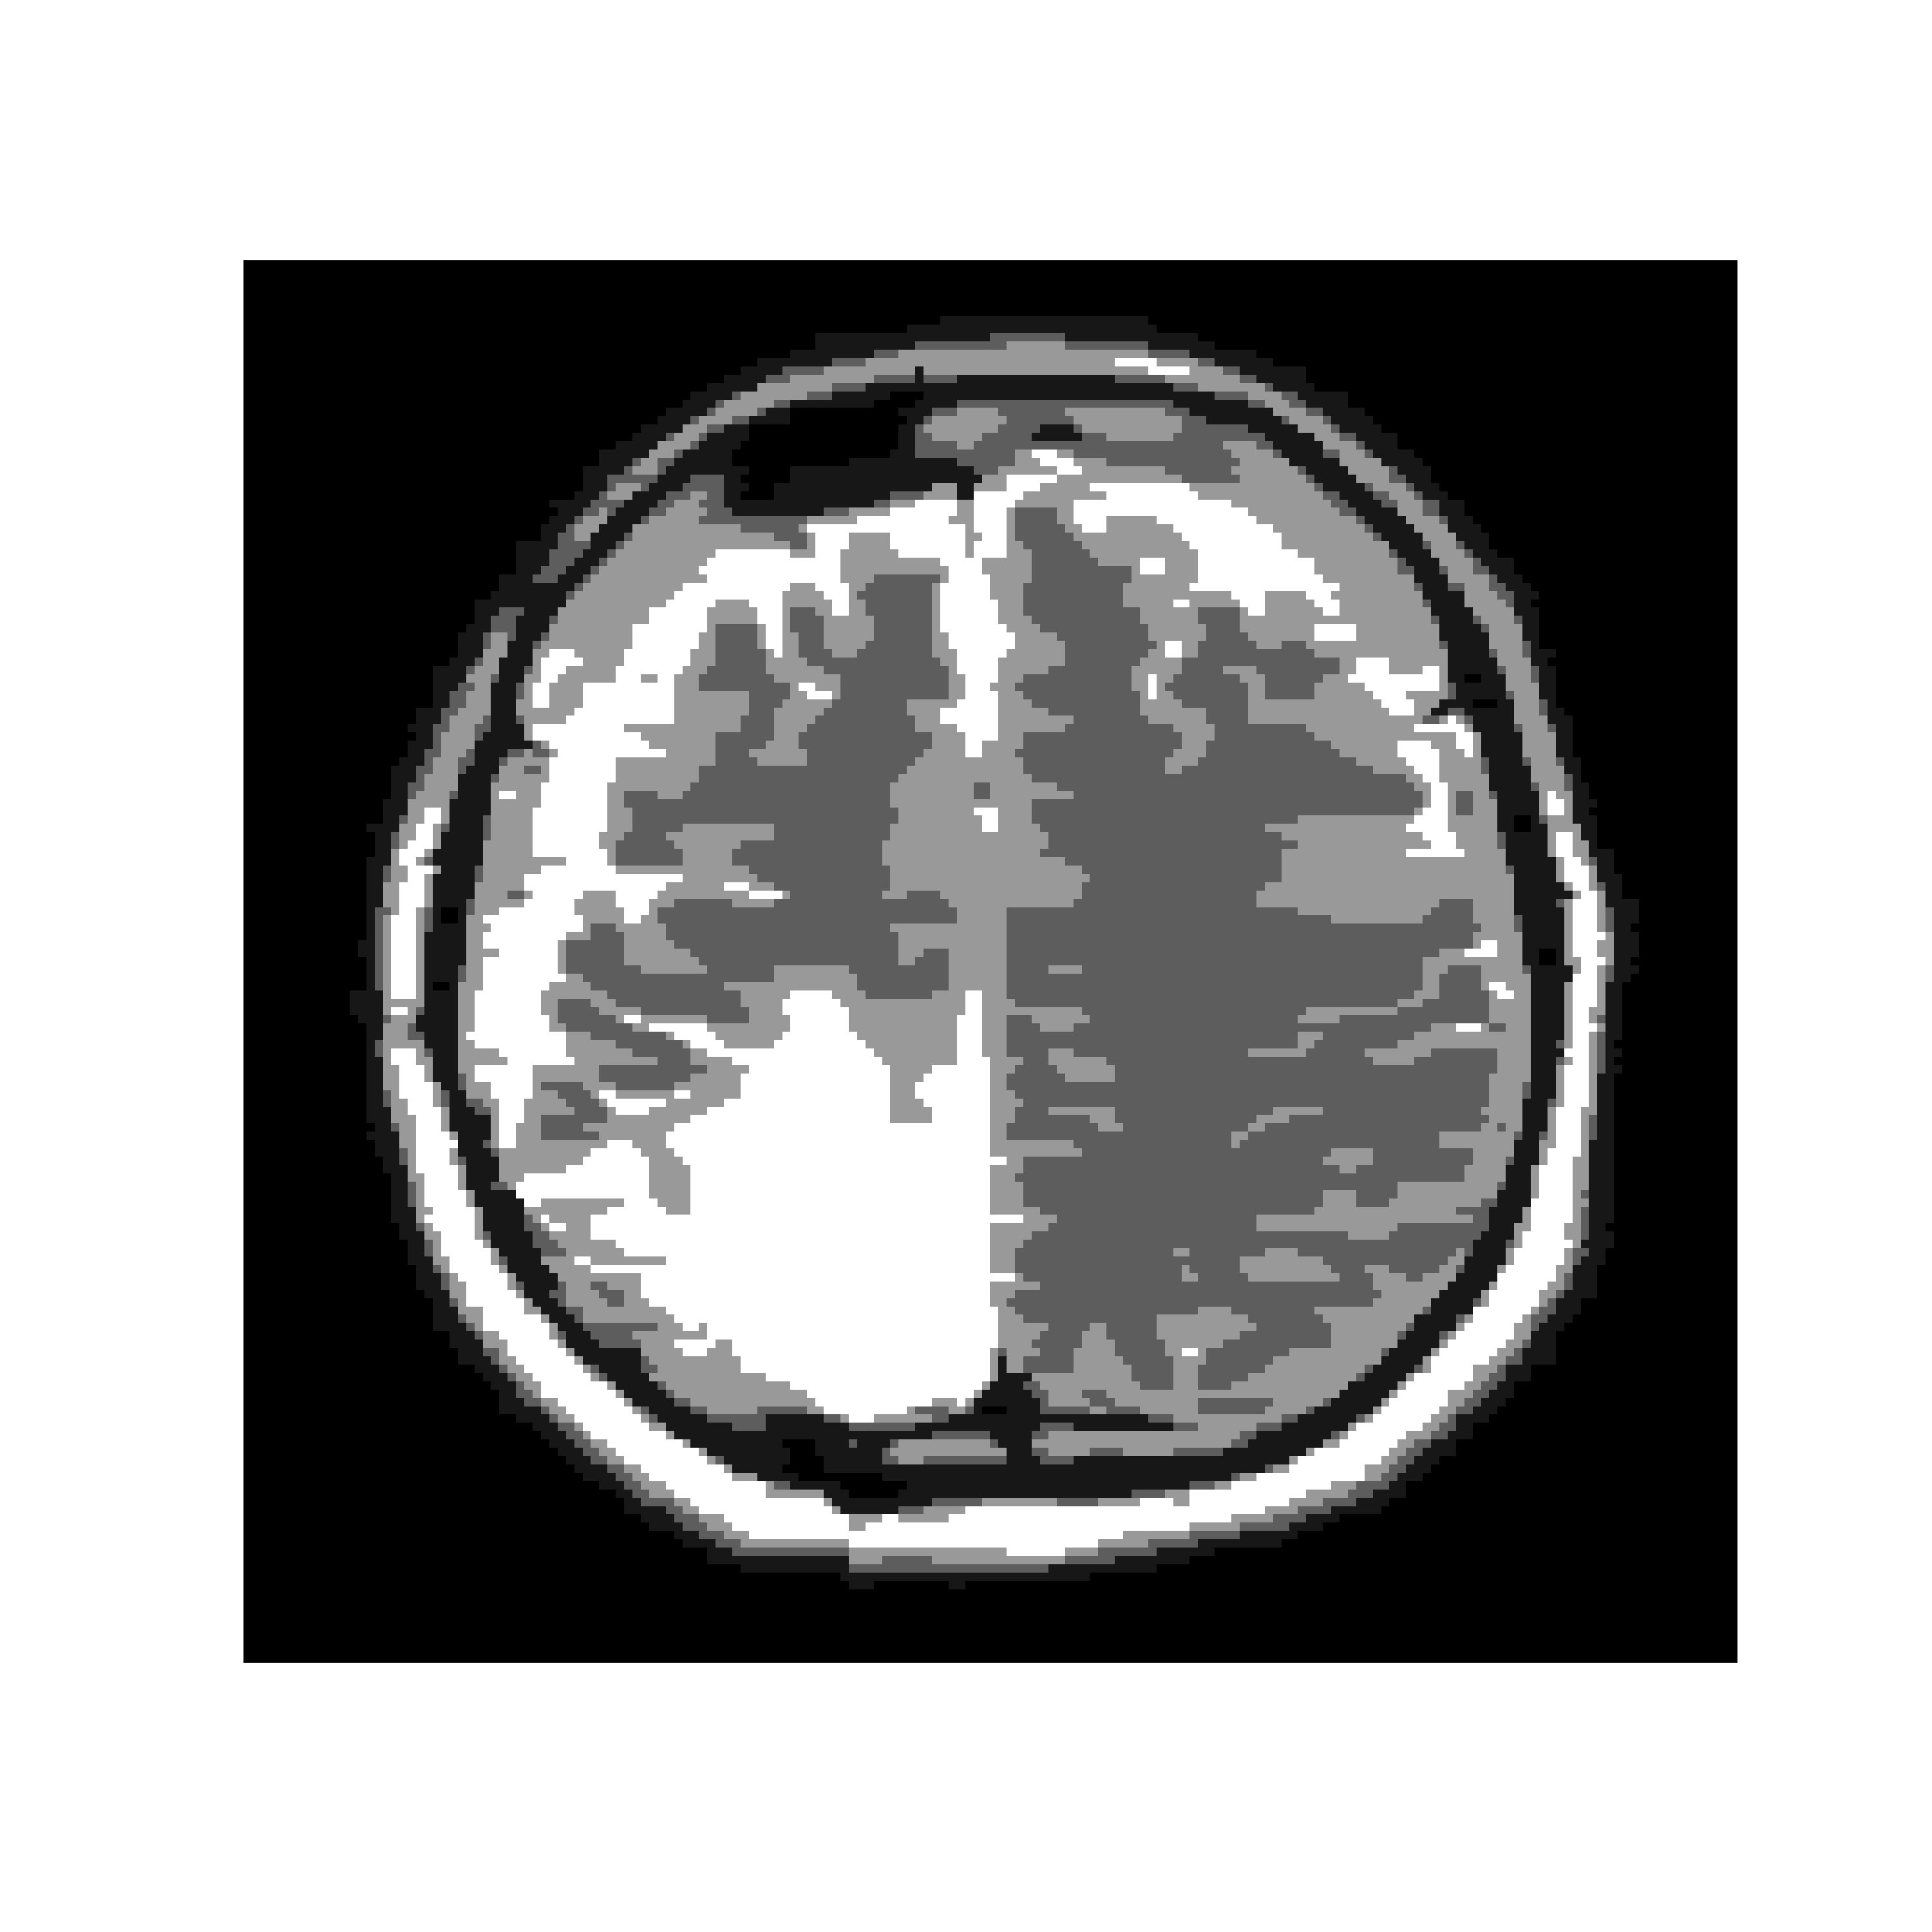
\includegraphics[width=0.3\textwidth]{../Cluster_results/MRI/MRI_hmm.png}}}
    \subfloat{{
\includegraphics[width=0.3\textwidth]{../Cluster_results/MRI/MRI_spec.png}}} \\ [-1em]
    \subfloat{{
\includegraphics[width=0.4\textwidth]{../Cluster_results/MRI/MRI_spec.png}}}%
    \subfloat{{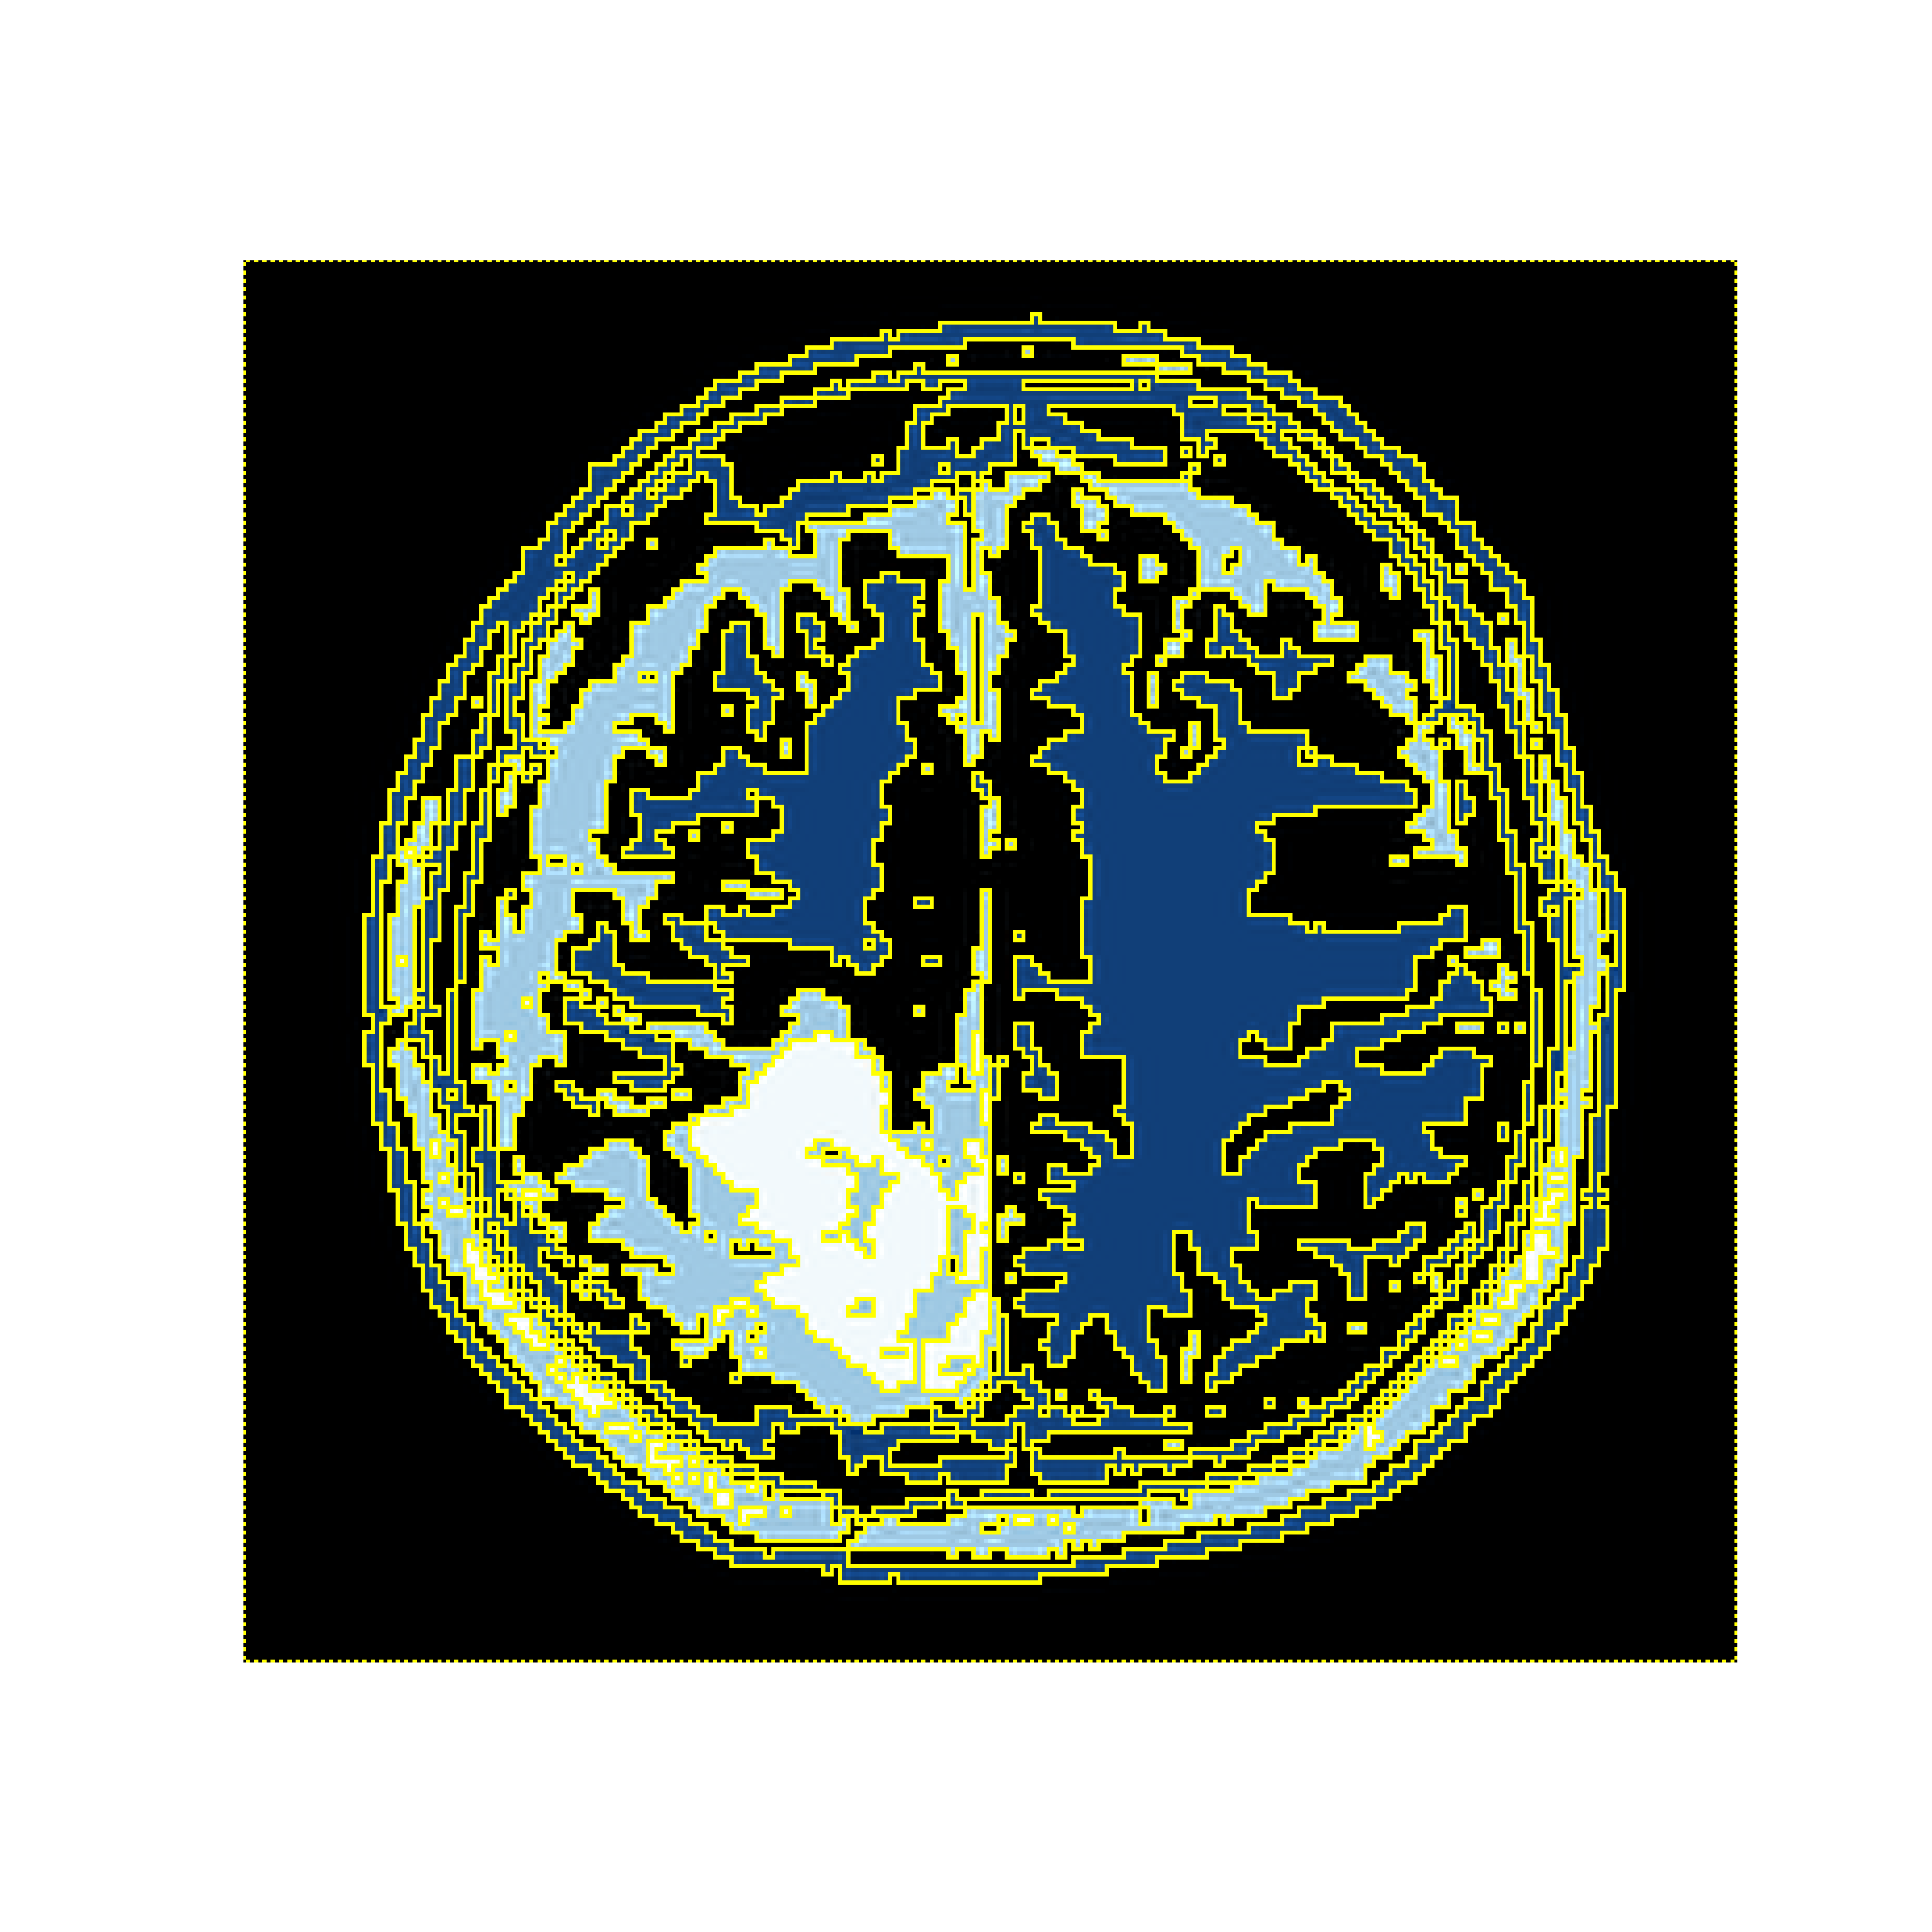
\includegraphics[width=0.4\textwidth]{../Cluster_results/MRI/MRI_spec_subpixel.png}}}
    \caption{The results obtained from K-means, HMM and spectral clustering from left to right.}
\end{figure}

%After demonstrating the power of spectral clustering, and limitations of k-means clustering and HMM in medical image segmentation. I decided to utilize only spectral clustering algorithm to segment a set of brain tumor images, which is obtained in \textit{Brain MRI Images for Brain Tumor Detection, Kaggle}.






\end{document}